\documentclass[]{article}
\usepackage{lmodern}
\usepackage{amssymb,amsmath}
\usepackage{ifxetex,ifluatex}
\usepackage{fixltx2e} % provides \textsubscript
\ifnum 0\ifxetex 1\fi\ifluatex 1\fi=0 % if pdftex
  \usepackage[T1]{fontenc}
  \usepackage[utf8]{inputenc}
\else % if luatex or xelatex
  \ifxetex
    \usepackage{mathspec}
  \else
    \usepackage{fontspec}
  \fi
  \defaultfontfeatures{Ligatures=TeX,Scale=MatchLowercase}
\fi
% use upquote if available, for straight quotes in verbatim environments
\IfFileExists{upquote.sty}{\usepackage{upquote}}{}
% use microtype if available
\IfFileExists{microtype.sty}{%
\usepackage{microtype}
\UseMicrotypeSet[protrusion]{basicmath} % disable protrusion for tt fonts
}{}
\usepackage[margin=1in]{geometry}
\usepackage{hyperref}
\hypersetup{unicode=true,
            pdftitle={Expanding tidy data principles to facilitate missing data exploration, visualization and assessment of imputations},
            pdfauthor={Nicholas Tierney, Department of Econometrics and Business Statistics, Monash University, Corresponding author (nicholas.tierney@gmail.com) Dianne Cook, Department of Econometrics and Business Statistics, Monash University},
            pdfborder={0 0 0},
            breaklinks=true}
\urlstyle{same}  % don't use monospace font for urls
\usepackage{color}
\usepackage{fancyvrb}
\newcommand{\VerbBar}{|}
\newcommand{\VERB}{\Verb[commandchars=\\\{\}]}
\DefineVerbatimEnvironment{Highlighting}{Verbatim}{commandchars=\\\{\}}
% Add ',fontsize=\small' for more characters per line
\usepackage{framed}
\definecolor{shadecolor}{RGB}{248,248,248}
\newenvironment{Shaded}{\begin{snugshade}}{\end{snugshade}}
\newcommand{\AlertTok}[1]{\textcolor[rgb]{0.94,0.16,0.16}{#1}}
\newcommand{\AnnotationTok}[1]{\textcolor[rgb]{0.56,0.35,0.01}{\textbf{\textit{#1}}}}
\newcommand{\AttributeTok}[1]{\textcolor[rgb]{0.77,0.63,0.00}{#1}}
\newcommand{\BaseNTok}[1]{\textcolor[rgb]{0.00,0.00,0.81}{#1}}
\newcommand{\BuiltInTok}[1]{#1}
\newcommand{\CharTok}[1]{\textcolor[rgb]{0.31,0.60,0.02}{#1}}
\newcommand{\CommentTok}[1]{\textcolor[rgb]{0.56,0.35,0.01}{\textit{#1}}}
\newcommand{\CommentVarTok}[1]{\textcolor[rgb]{0.56,0.35,0.01}{\textbf{\textit{#1}}}}
\newcommand{\ConstantTok}[1]{\textcolor[rgb]{0.00,0.00,0.00}{#1}}
\newcommand{\ControlFlowTok}[1]{\textcolor[rgb]{0.13,0.29,0.53}{\textbf{#1}}}
\newcommand{\DataTypeTok}[1]{\textcolor[rgb]{0.13,0.29,0.53}{#1}}
\newcommand{\DecValTok}[1]{\textcolor[rgb]{0.00,0.00,0.81}{#1}}
\newcommand{\DocumentationTok}[1]{\textcolor[rgb]{0.56,0.35,0.01}{\textbf{\textit{#1}}}}
\newcommand{\ErrorTok}[1]{\textcolor[rgb]{0.64,0.00,0.00}{\textbf{#1}}}
\newcommand{\ExtensionTok}[1]{#1}
\newcommand{\FloatTok}[1]{\textcolor[rgb]{0.00,0.00,0.81}{#1}}
\newcommand{\FunctionTok}[1]{\textcolor[rgb]{0.00,0.00,0.00}{#1}}
\newcommand{\ImportTok}[1]{#1}
\newcommand{\InformationTok}[1]{\textcolor[rgb]{0.56,0.35,0.01}{\textbf{\textit{#1}}}}
\newcommand{\KeywordTok}[1]{\textcolor[rgb]{0.13,0.29,0.53}{\textbf{#1}}}
\newcommand{\NormalTok}[1]{#1}
\newcommand{\OperatorTok}[1]{\textcolor[rgb]{0.81,0.36,0.00}{\textbf{#1}}}
\newcommand{\OtherTok}[1]{\textcolor[rgb]{0.56,0.35,0.01}{#1}}
\newcommand{\PreprocessorTok}[1]{\textcolor[rgb]{0.56,0.35,0.01}{\textit{#1}}}
\newcommand{\RegionMarkerTok}[1]{#1}
\newcommand{\SpecialCharTok}[1]{\textcolor[rgb]{0.00,0.00,0.00}{#1}}
\newcommand{\SpecialStringTok}[1]{\textcolor[rgb]{0.31,0.60,0.02}{#1}}
\newcommand{\StringTok}[1]{\textcolor[rgb]{0.31,0.60,0.02}{#1}}
\newcommand{\VariableTok}[1]{\textcolor[rgb]{0.00,0.00,0.00}{#1}}
\newcommand{\VerbatimStringTok}[1]{\textcolor[rgb]{0.31,0.60,0.02}{#1}}
\newcommand{\WarningTok}[1]{\textcolor[rgb]{0.56,0.35,0.01}{\textbf{\textit{#1}}}}
\usepackage{longtable,booktabs}
\usepackage{graphicx,grffile}
\makeatletter
\def\maxwidth{\ifdim\Gin@nat@width>\linewidth\linewidth\else\Gin@nat@width\fi}
\def\maxheight{\ifdim\Gin@nat@height>\textheight\textheight\else\Gin@nat@height\fi}
\makeatother
% Scale images if necessary, so that they will not overflow the page
% margins by default, and it is still possible to overwrite the defaults
% using explicit options in \includegraphics[width, height, ...]{}
\setkeys{Gin}{width=\maxwidth,height=\maxheight,keepaspectratio}
\IfFileExists{parskip.sty}{%
\usepackage{parskip}
}{% else
\setlength{\parindent}{0pt}
\setlength{\parskip}{6pt plus 2pt minus 1pt}
}
\setlength{\emergencystretch}{3em}  % prevent overfull lines
\providecommand{\tightlist}{%
  \setlength{\itemsep}{0pt}\setlength{\parskip}{0pt}}
\setcounter{secnumdepth}{5}
% Redefines (sub)paragraphs to behave more like sections
\ifx\paragraph\undefined\else
\let\oldparagraph\paragraph
\renewcommand{\paragraph}[1]{\oldparagraph{#1}\mbox{}}
\fi
\ifx\subparagraph\undefined\else
\let\oldsubparagraph\subparagraph
\renewcommand{\subparagraph}[1]{\oldsubparagraph{#1}\mbox{}}
\fi

%%% Use protect on footnotes to avoid problems with footnotes in titles
\let\rmarkdownfootnote\footnote%
\def\footnote{\protect\rmarkdownfootnote}

%%% Change title format to be more compact
\usepackage{titling}

% Create subtitle command for use in maketitle
\newcommand{\subtitle}[1]{
  \posttitle{
    \begin{center}\large#1\end{center}
    }
}

\setlength{\droptitle}{-2em}

  \title{Expanding tidy data principles to facilitate missing data exploration,
visualization and assessment of imputations}
    \pretitle{\vspace{\droptitle}\centering\huge}
  \posttitle{\par}
    \author{Nicholas Tierney, Department of Econometrics and Business Statistics,
Monash University, \textbf{Corresponding author
(\href{mailto:nicholas.tierney@gmail.com}{\nolinkurl{nicholas.tierney@gmail.com}})}
\newline Dianne Cook, Department of Econometrics and Business
Statistics, Monash University}
    \preauthor{\centering\large\emph}
  \postauthor{\par}
      \predate{\centering\large\emph}
  \postdate{\par}
    \date{September 6, 2018}

%% Any special functions or other packages can be loaded here.


%% FIGURE FLOATING taken from
%% https://stackoverflow.com/questions/16626462/figure-position-in-markdown-when-converting-to-pdf-with-knitr-and-pandoc
\usepackage{float}
\let\origfigure\figure
\let\endorigfigure\endfigure
\renewenvironment{figure}[1][2] {
    \expandafter\origfigure\expandafter[H]
} {
    \endorigfigure
}

%% MONASH STUFF TAKEN FROM ROB

%% SPACING
\RequirePackage{setspace}
\spacing{1.5}


%% HEADERS AND FOOTERS
\RequirePackage{fancyhdr}
\pagestyle{fancy}
\rfoot{\Large\sffamily\raisebox{-0.1cm}{\textbf{\thepage}}}
\makeatletter
\lhead{\textsf{\expandafter{\@title}}}
\makeatother
\rhead{}
\cfoot{}
\setlength{\headheight}{15pt}
\renewcommand{\headrulewidth}{0.4pt}
\renewcommand{\footrulewidth}{0.4pt}
\fancypagestyle{plain}{%
\fancyhf{} % clear all header and footer fields
\fancyfoot[C]{\sffamily\thepage} % except the center
\renewcommand{\headrulewidth}{0pt}
\renewcommand{\footrulewidth}{0pt}}

%% LINE AND PAGE BREAKING
\sloppy
\clubpenalty = 10000
\widowpenalty = 10000
\brokenpenalty = 10000
\RequirePackage{microtype}

%% PARAGRAPH BREAKS
\setlength{\parskip}{1.4ex}
\setlength{\parindent}{0em}

%% CAPTIONS
\RequirePackage{caption}
\DeclareCaptionStyle{italic}[justification=centering]
 {labelfont={bf},textfont={it},labelsep=colon}
\captionsetup[figure]{style=italic,format=hang,singlelinecheck=true}
\captionsetup[table]{style=italic,format=hang,singlelinecheck=true}
\usepackage{booktabs}
\usepackage{longtable}
\usepackage{array}
\usepackage{multirow}
\usepackage[table]{xcolor}
\usepackage{wrapfig}
\usepackage{float}
\usepackage{colortbl}
\usepackage{pdflscape}
\usepackage{tabu}
\usepackage{threeparttable}
\usepackage{threeparttablex}
\usepackage[normalem]{ulem}
\usepackage{makecell}

\usepackage{amsthm}
\newtheorem{theorem}{Theorem}[section]
\newtheorem{lemma}{Lemma}[section]
\theoremstyle{definition}
\newtheorem{definition}{Definition}[section]
\newtheorem{corollary}{Corollary}[section]
\newtheorem{proposition}{Proposition}[section]
\theoremstyle{definition}
\newtheorem{example}{Example}[section]
\theoremstyle{definition}
\newtheorem{exercise}{Exercise}[section]
\theoremstyle{remark}
\newtheorem*{remark}{Remark}
\newtheorem*{solution}{Solution}
\begin{document}
\maketitle

\textbf{Abstract}:

Despite the large body of research on missing value distributions and
imputation, there is comparatively little literature on how to make it
easy to handle, explore, and impute missing values in data. This paper
addresses this gap. The new methodology builds upon tidy data
principles, with a goal to integrating missing value handling as an
integral part of data analysis workflows. New data structures are
defined along with new functions (verbs) to perform common operations.
Together these provide a cohesive framework for handling, exploring, and
imputing missing values. These methods have been made available in the R
package \texttt{naniar}.

\emph{Keywords:} workflow, statistical computing, data science, data
visualization, tidyverse, data pipeline

\newpage

\hypertarget{intro}{%
\section{Introduction}\label{intro}}

Tidy data (Wickham 2014) is a relatively new principle and suite of
tools that facilitate the process of converting raw data into a clean,
analysis-ready format that works efficiently in a data analysis
pipeline. In tidy data, missing values can be handled implicitly or
explicitly, at the analyst's discretion. However, when making a plot,
missing values are simply dropped, albeit with a warning (see Figure
\ref{fig:warning}). Most other analysis software will simply drop cases
with missings without warning.

\begin{figure}

{\centering 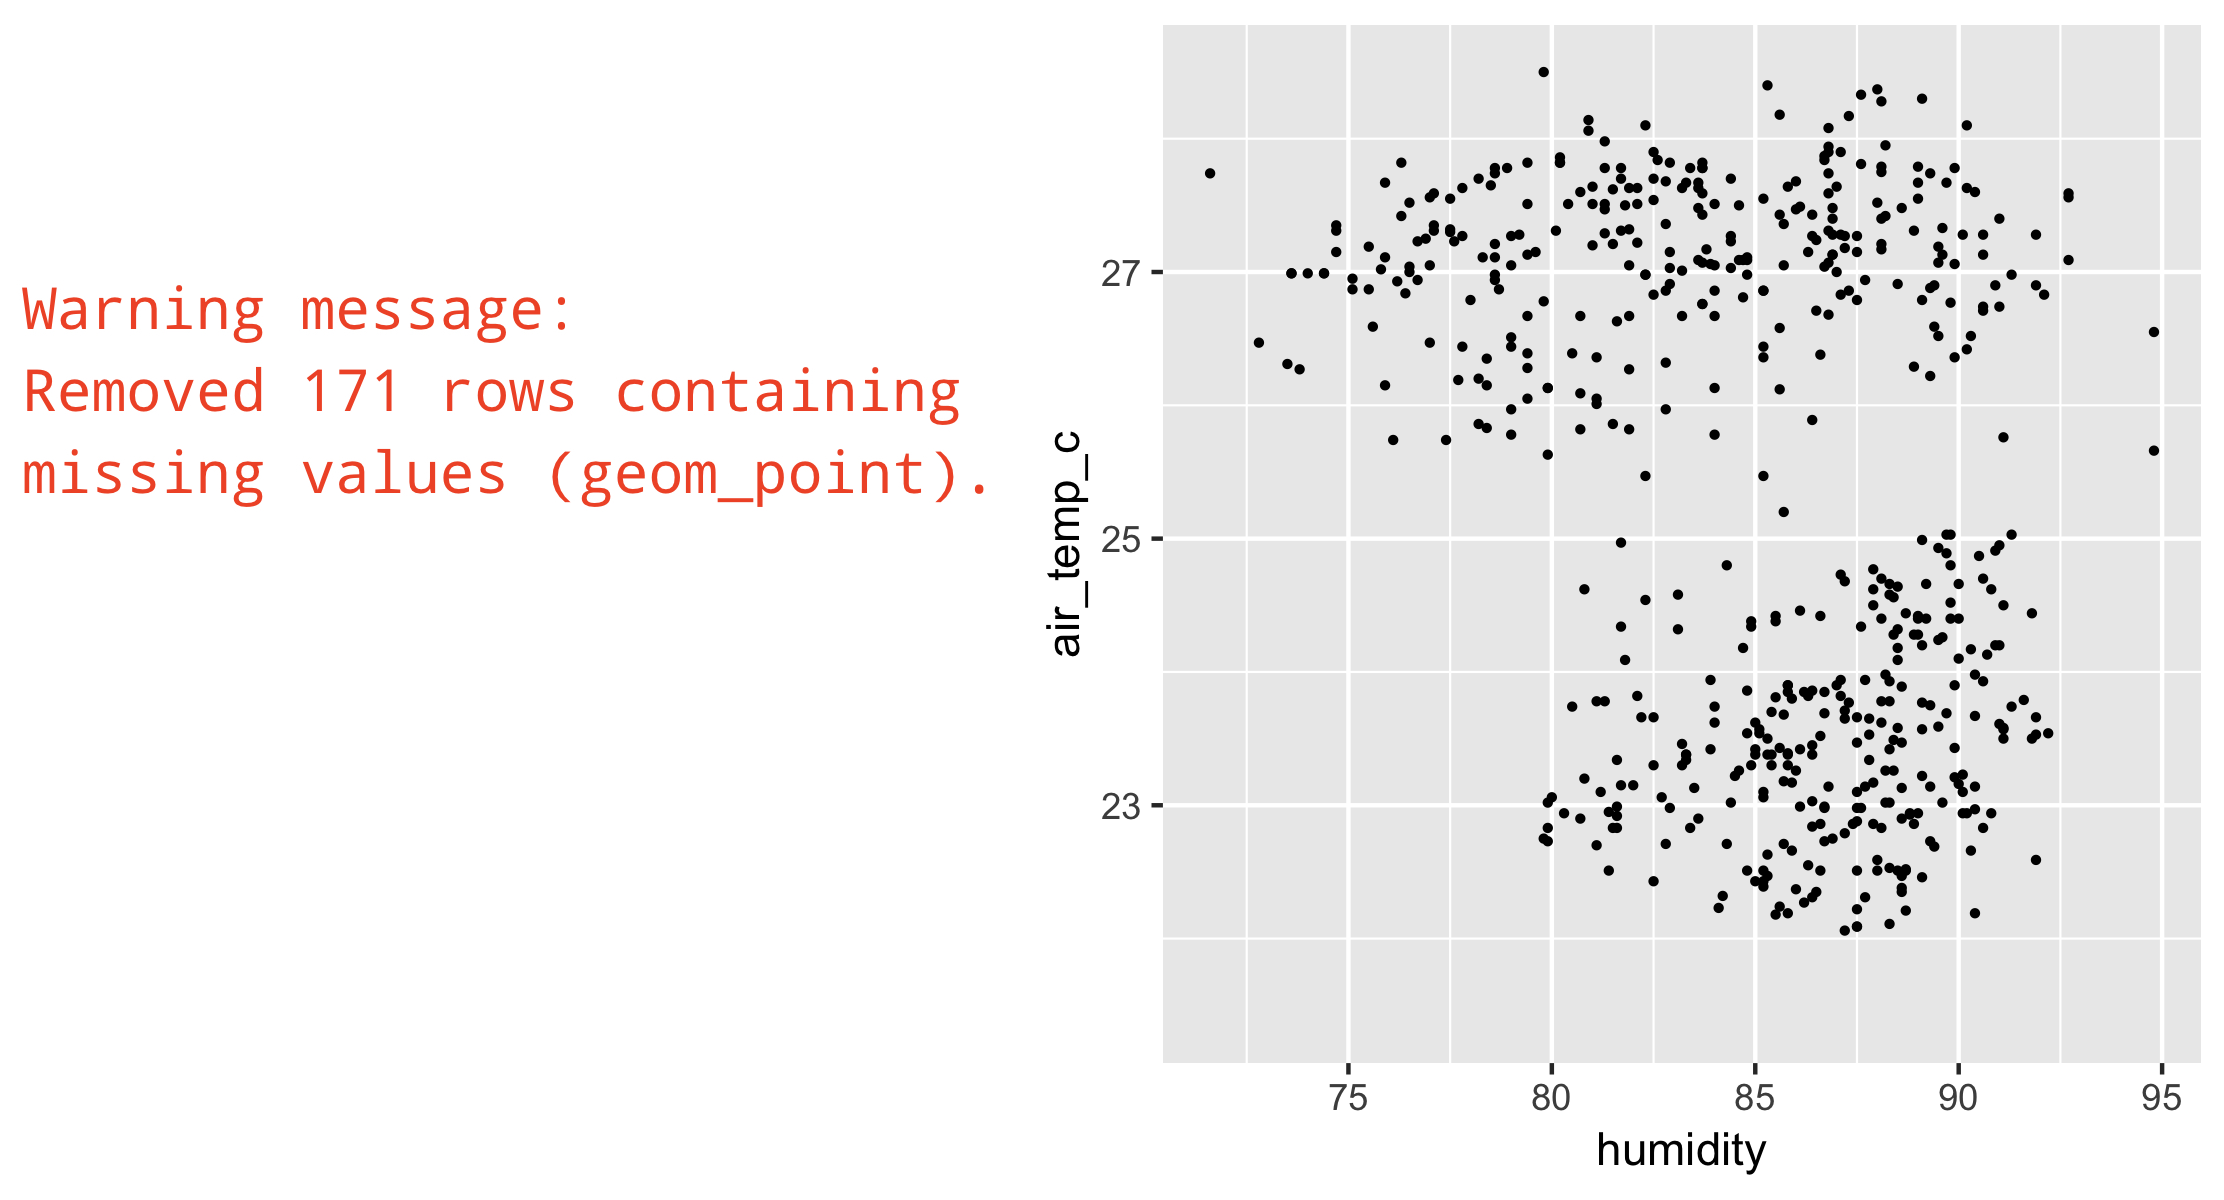
\includegraphics[width=1\linewidth]{ggplot2-warning-and-plot} 

}

\caption{How ggplot behaves when displaying missing values:  Warning message (Left) is thrown prior to plot (Right); ggplot2 does not display missing values in the plot, but at least throws a warning message to the user, which is better than many statistical models.}\label{fig:warning}
\end{figure}

The imputation literature does not address how to handle missing data.
Producing a complete dataset for analysis, whether by case or variable
deletion, or with imputation, requires knowing something about the
structure of the missing values. To understand their structure, one
needs to generate visualizations, calculate summaries, and perform
exploratory modelling. The imputation methods literature (e.g. Little
(1988), Rubin (1976), Simon and Simonoff (1986), Schafer and Graham
(2002), Buuren (2012)) focuses on ensuring valid statistical inference
is made from incomplete data. They approach this chiefly through
probabilistic modelling, and assume the mechanism of missing data is
known to the analyst.

Exploring missing data to find the missingness mechanism is difficult,
because it is an iterative process with many dead ends and often no
clear answer. There is no silver bullet for missing data that will
reveal it's mechanism to the analyst. Despite it being crucial to
explore and understand missing data, there is very little research on
how to make this process more efficient so that it integrates into
analysis pipelines. Although decision tree models or latent group
analysis can reveal structures or patterns of missingness (Barnett et
al. 2017; Tierney et al. 2015), these are not definitive and usually
require discussion with data curators to validate. The analyst must
explore missing data using visualizations, summaries, and exploratory
analyses, but there is a lack of tools to efficiently explore missing
data.

The graphics literature (Swayne and Buja 1998; Unwin et al. 1996)
provides several solutions for exploring missings visually. These
approaches incorporate missings into the plot in some way. For example,
imputing values 10\% below the range to display all values in a scatter
plot. These methods require the data to be linked to the missing or
imputed values; this link is typically hidden from the user. The
approaches from the graphics literature have not been translated and
integrated into tidy data. This limits the analysts capacity to
efficiently explore missing values. Extending tidy data and tidy tools
to account for missing values would create more efficient and robust
workflows and analysis.

The paper is organized in the following way to discuss the problem of
missing data. The next section (\ref{tidy-data-concepts}) is an
introduction to tidy data principles and tools. Missing value imputation
(\ref{missing-data-rep-dep} and \ref{imputation}) and exploration
literature (\ref{exploration}) are then discussed. Section
\ref{extensions} discusses extensions to the tidy methodology that
facilitates operations for exploring, visualizing, and imputing missing
data. The application of these new methods is illustrated using a case
study in section \ref{case-study}. Finally, section \ref{discussion}
discusses strengths, limitations, and future directions.

\hypertarget{background}{%
\section{Background}\label{background}}

\hypertarget{tidy-data-concepts}{%
\subsection{Tidy data concepts and methods}\label{tidy-data-concepts}}

Features of tidy data were formally discussed in 2014 (Wickham 2014),
subsequently generating much discussion (see Donoho (2017) and
commentary), and tools for data analysis. Tidy data is defined as:

\begin{quote}
\begin{enumerate}
\def\labelenumi{\arabic{enumi}.}
\tightlist
\item
  Each variable forms a column.
\item
  Each observation forms a row.
\item
  Each type of observational unit forms a table.
\end{enumerate}
\end{quote}

Tidy data is easier to work with and analyze because the variables are
in the same format as they would be put into modelling software. This
helps the analyst works swiftly and clearly, closing up opportunities
for errors.

With tidy data come tidy tools, which have the same input and output:
tidy data. This consistency means multiple tools can be composed
together in sequence, allowing for rapid, elegant operations.
Contrasting tidy tools are messy tools. These have tidy input but messy
output. Messy tools slow down analysis by shifting the focus from
analysis to transforming output so it is the right shape for the next
step in the analysis. This makes the work at each step harder to
predict, and more complex and difficult to maintain. This disrupts
workflow, and incites errors.

Tidy tools fall into three broad categories: data manipulation,
visualization, and modelling. These are now discussed in turn.

\hypertarget{tidy-data-manip}{%
\subsubsection{Data manipulation}\label{tidy-data-manip}}

Data manipulation is made input and output tidy with R packages
\texttt{dplyr} and \texttt{tidyr} (Wickham et al. 2017a; Wickham and
Henry 2018). These provide the five ``verbs'' of data manipulation: data
reshaping, sorting, filtering, transforming, and aggregating.
\textbf{Data reshaping} goes from long to wide formats; \textbf{sorting}
arranges rows in a specific order; \textbf{filtering} removes rows based
on a condition; \textbf{transforming} changes existing variables or
adding new ones; \textbf{aggregating} creates a single value from many
values, say for example by computing the minimum, maximum, and mean.

\hypertarget{tidy-vis}{%
\subsubsection{Visualizations}\label{tidy-vis}}

Visualization tools only have tidy data as their input, as the output is
a graphic. The popular domain specific language \texttt{ggplot2} maps
variables in a dataset to features (referred to as aesthetics) of a
graphic (Wickham 2009). For example, a scatterplot can be created by
mapping two variables to the x and y axes, and specifying a point
geometry. The graph can then be changed to map a third variable to color
of the points, and a fourth variable to size.

\hypertarget{tidy-model}{%
\subsubsection{Modelling}\label{tidy-model}}

Modelling tools work well with tidy data, as they have a clear mapping
from variables in the data to the formula for a model. For example in R,
y regressed on x and z is: \texttt{lm(y\ \textasciitilde{}\ x\ +\ z)}.
Modelling tools are input tidy, but their output is always messy. For
example, estimated coefficients, predictions, and residuals from one
model cannot be easily combined with the output of another model. The
\texttt{recipes} package is a tidy tool under development to help make
modelling input and output tidy (Kuhn and Wickham 2018).

\hypertarget{the-tidyverse}{%
\subsubsection{The tidyverse}\label{the-tidyverse}}

Defining tidy data and tidy tools has resulted in the growth of a set of
packages known collectively as the ``tidyverse'' (Ross et al. 2017).
These are designed to share similar principles in their design and
behavior, and cover the breadth of an analysis - going from importing,
tidying, transforming, visualizing, modelling, to communicating (Ross et
al. 2017; Wickham 2017; Wickham and Grolemund 2016). This has led to a
growth of tools for specific parts of analysis - from reading in data
with \texttt{readr}, \texttt{readxl}, and \texttt{haven}, to handling
character strings with \texttt{stringr}, dates with \texttt{lubridate},
and performing functional programming with \texttt{purrr} (Grolemund and
Wickham 2011; Henry and Wickham 2017; Wickham 2018; Wickham and Bryan
2017; Wickham et al. 2017b; Wickham and Miller 2018). It has also led to
the growth of new packages for other fields that follow similar design
principles and create fluid workflows for new domains. For example, the
\texttt{tidytext} package for text analysis, the \texttt{tsibble}
package for time series data, and \texttt{tidycensus} for working with
US census and boundary data (Silge and Robinson 2016; Walker 2018; Wang
et al. 2018).

\hypertarget{tidy-formats-missing-data}{%
\subsubsection{Tidy formats for missing
data}\label{tidy-formats-missing-data}}

Current tools for missing data are messy. Missing data tools can be used
to perform imputations, missing data diagnostics, and data
visualizations. However, these tools are primarily \emph{messy}, and
suffer the same problems as modelling for imputation: They use tidy
input, but produce messy output. The complex, often multivariate nature
of imputation methods also makes makes them difficult to represent.
Visualization methods for missing data do not map data features to the
aesthetics of a graphic, as in \texttt{ggplot2}, limiting expressive
exploration.

Past graphics research on missing data has not yet been framed in a tidy
way. The graphics literature has explored methods for missing value
exploration and imputation. Translating and expanding these to fit
within tidy data and tidy tools would create more efficient workflows.

\hypertarget{missing-data-rep-dep}{%
\subsection{Missing data representation and
dependence}\label{missing-data-rep-dep}}

The information on missing values in a dataset can be represented as a
missingness matrix, \(R\), where 0 is observed data and 1 is missing
data, where for data \(y\) with \(i\) rows and \(j\) columns, the value
\(r_{ij}\) is given by:

\[
r_{ij} =\begin{cases}
1, & \text{if } y_{ij} \text{ is missing} \\
0, & \text{if } y_{ij} \text{ is observed}
\end{cases}
\]

There are many ways each value can go missing. The information in \(R\)
can be used to arrive at three categories of missing values: Missing
completely at random (MCAR), Missing at random, and missing not at
random. \textbf{MCAR} is where values being missing have no association
with observed or unobserved data, that is
\(Pr(missing | observed, unobserved) = Pr(missing)\). Essentially, the
probability of an observation being missing is unrelated to anything
else. Although this is a convenient scenario, it is not actually
possible to confirm, as it relies on statements on data unobserved.
\textbf{MAR} refers to cases where the missingness only depends on the
data observed, and not data unobserved, that
is,\(Pr(missing | observed, unobserved) = Pr(missing | observed)\). Some
structure or dependence between the missing values and observed values
is allowed, provided that this can be explained by the data observed.
Finally, \textbf{MNAR} refers to the missingness being related to values
unobserved: \(Pr(missing | observed, unobserved)\). This assumes that
conditioning on all available observed data, the data goes missing due
to some phenomena unobserved. This presents a challenge in analysis, as
it is difficult to verify this state, and also implies bias in analysis
due to the unobserved phenomena.

Visualizations can help assess whether data is MCAR, MAR or MNAR.
Imputation is recommended in most cases of missingness dependence, where
the values are plausible (e.g., imputing a pulse for someone deceased),
as this can help re-assess the classification of missingness.

\hypertarget{imputation}{%
\subsection{Imputation}\label{imputation}}

Imputation methods are more accessible than they have ever been, and the
number of methods and implementations in software continues to grow.
Values can be imputed with one value (single imputation), or multiple
values (multiple imputation), creating \(m\) datasets. Methods and
software for single and multiple imputation are now discussed.

\hypertarget{single-imputation}{%
\subsubsection{Single imputation}\label{single-imputation}}

\texttt{VIM} (Kowarik and Templ 2016) efficiently implements well-used
imputation methods k-nearest neighbor, regression, hot-deck, and
iterative robust model-based imputation. This diversity of approaches
allow the package to deal semi-continuous, continuous, count, and
categorical data. VIM identifies imputed cases by adding an indicator
variable with a suffix \texttt{\_imp}. So \texttt{Var1} would have a
sibling indicator column, \texttt{Var1\_imp}, with TRUE or FALSE values
to indicate imputed value. \texttt{VIM} also has a variety of
visualization methods, discussed in section \ref{exploration}. The
\texttt{simputation} package includes imputation methods for linear
regression, decision trees, K nearest neighbors, hotdeck imputation, and
the EM algorithm (Dempster et al. 1977; van der Loo 2017). A key feature
of its design is that it returns a regular dataframe. This approach
contrasts from other imputation software, which may provide custom
classes of data or additional objects, which require additional work to
prepare for subsequent analysis. Providing a dataframe with imputed
values included in the data reduces the friction of working with other
tools, but comes at the cost identifying imputed values. Other software
for imputation includes \texttt{Hmisc} (Harrell Jr et al. 2018), which
provide predictive mean matching, \texttt{imputeTS} (Moritz and
Bartz-Beielstein 2017), which provide time series imputation methods,
and \texttt{missMDA} (Josse and Husson 2016), which imputes data using
principal components analysis.

\hypertarget{multiple-imputation}{%
\subsubsection{Multiple imputation}\label{multiple-imputation}}

Multiple imputation is often regarded as best practice for imputing
values (Schafer and Graham 2002), as long as appropriate caution is
taken (Sterne et al. 2009). Popular and robust methods for multiple
imputation include the \texttt{mice}, \texttt{Amelia}, and \texttt{mi}
packages (Gelman and Hill 2011; Honaker et al. 2011; van Buuren and
Groothuis-Oudshoorn 2011). The \texttt{mice} package implements the
method of chained equations, using a variable-wise algorithm to
calculate the posterior distribution of parameters, from which uses to
generate imputed values. The suggested workflow in \texttt{mice}
revolves around imputing data, returning completed data, and fitting a
model and pooling the results. The \texttt{Amelia} package (Honaker et
al. 2011) assumes data are multivariate normal, and samples from the
posterior using the computationally efficient (and parallelizable)
Expectation-Maximization Bootstrap (EMB) algorithm (Honaker and King
2010) and allows for incorporation of information on the values in a
prior. The \texttt{mi} package (Gelman and Hill 2011) also uses Bayesian
models for imputation, providing better handling of semi-continuous
values, and data with structural or perfect correlation. A collection of
analysis models are also provided in \texttt{mi}, which work with the
specially multiply imputed data, including linear models, generalized
linear models, and their corresponding Bayesian components. This
approach promotes fluid workflow, with a similar penalty to tidying up
model output, which is still messy. Another software for performing
multiple imputation is \texttt{norm} (R by Alvaro A. Novo. Original by
Joseph L. Schafer \textless{}jls@stat.psu.edu\textgreater{}. 2013;
Schafer 1999), which uses methods from the NORM software from Schafer
(1999), such as multiple imputations using EM for multivariate normal
data. The \texttt{norm} package does not provide a framework for
tracking missing values, but instead provides tools for making inference
from multiple imputation. Each of these multiple imputation methods
provide practical methods, but do not have consistent interfaces across
their methods or implementation, which makes then inherently messy, as
their output is always different. A consistent data structure that
tracks missing values by default would make the data outputs tidy,
streamlining subsequent analysis.

\hypertarget{exploration}{%
\subsection{Exploration}\label{exploration}}

The primary focus of most missing data packages is exploring imputed
values, not on exploring relationships in missing values, and
identifying possible patterns. Texts that do cover exploration of
missing data have the same problem as with modelling: the input is tidy,
but the output is messy and does not work with other tools (Buuren
2012); this is inefficient. Methods for exploring missing values are
primarily covered in literature on interactive graphics (Cook and Swayne
2007; Swayne and Buja 1998; Unwin et al. 1996), and are picked up again
in a discussion of a graphical user interface (Cheng et al. 2015).

Missing values in a dataset can be represented as a binary matrix where
0 is present and 1 is missing (Rubin 1976; Schafer and Graham 2002).
This is often referred to as a matrix \(R\), which can be used to assess
missing data dependence. This idea of a matrix of missing values has
also been used in interactive graphics, dubbed a ``shadow matrix'', to
link missing and imputed values to the data, facilitating their display
in graphics (Swayne and Buja 1998). This work also focuses heavily on
multivariate numeric data. This is an idea upon which this new work
builds.

The approach of Unwin et al. (1996) focussed on multivariate categorical
data, where missingness is explicitly added as an additional category.
MANET also provided univariate visualizations of missing data using
linked brushing between a reference plot of the missingness for each
variable, and a plot of the data as a histogram or barplot. The approach
of Swayne and Buja (1998) in the software XGobi, further developed in
ggobi (Cook and Swayne 2007), focussed more on multivariate quantitative
data. Missingness is incorporated into plots in ggobi by setting them to
be 10\% below the minimum value.

MissingDataGUI provides a user interface for exploring missing data
structure both numerically and visually. Using a GUI to explore missing
data may make it easier to glean valuable insight into important
structures for missingness. However, these insights are typically not
captured or recorded, so it is difficult to incorporate them into
reproducible analyses. This distracts and breaks analysis workflow,
inviting mistakes.

VIM (visualizing and Imputing Missing Data) provides visualization
methods that identify observed, imputed, and missing values. These
include spinograms, spinoplots, missingness matrices, plotting
missingness in the margins of other plots, and other summaries. These
help explore missingness, however these visualizations do not map
variables to graphical aesthetics, creating friction moving across
workflows, making them difficult to extend to new circumstances.
Additionally, data used to create the visualizations cannot be accessed,
posing a barrier to further explorations.

\texttt{ggplot2} incorporates missingness into visualizations only when
mapping a discrete variable to a graph aesthetic. This has some
limitations. For example, for data with school grades and test scores, a
boxplot visualization could have school grade mapped to the x axis, and
test score to the y axis (See Figure \ref{fig:gg-box-na}). If there are
missings in a continuous variable like test score, \texttt{ggplot2}
omits the missing values and prints a warning message. However, if a
discrete variable like school year has missing values, an NA category is
created for school year, and the scores are placed into this.

Figure \ref{fig:gg-box-na}, shows four scenarios of missingness for test
scores across school year - the first contains no missingness, the
second contains missingness for school year, the third contains
missingness in scores, and the fourth contains missingness in both.

\begin{figure}

{\centering 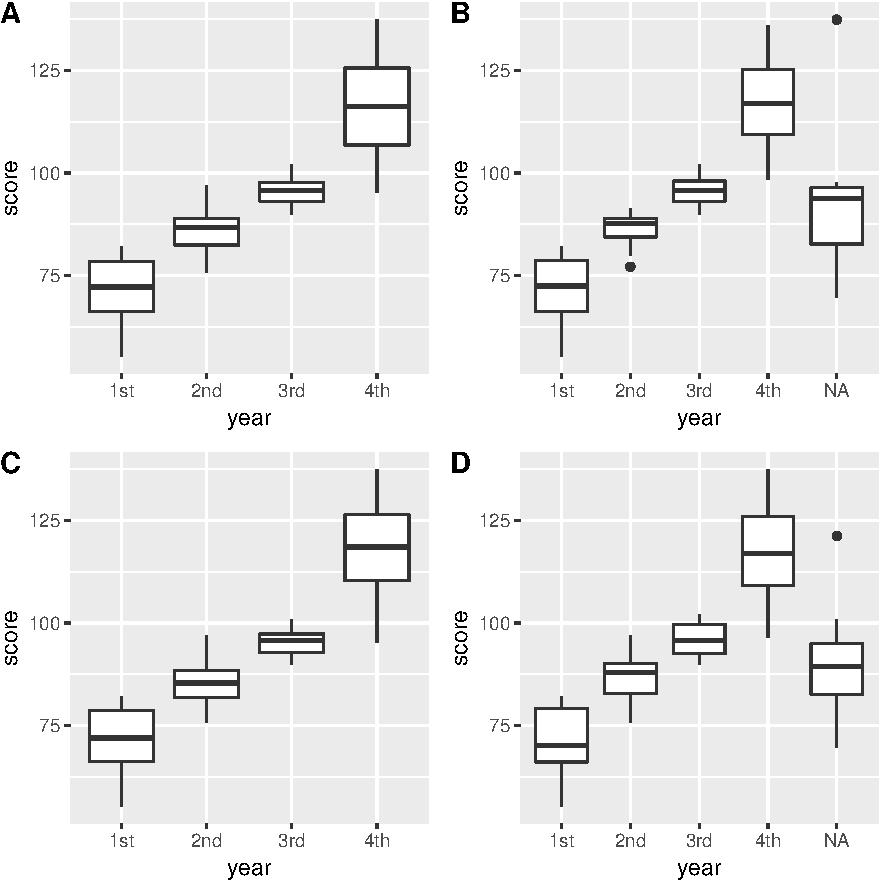
\includegraphics[width=0.7\linewidth]{tidy-missing-data-paper_files/figure-latex/gg-box-na-1} 

}

\caption{ggplot2 provides different visualizations depending on what type of data has missing values. (A) Data is complete and graphic is presented; (B) Missings are only in category variable year - an additional 'NA' boxplot is created; (C) Missings only in scores, no additional missingness information is shown; (D) Missings in both scores and school year, additional missing information is shown. The missingness category is only shown when there are missings in categorical variables such as year (plots (B) and (D)). In (C), no missingness information is given on the graphic, despite there being missings in score, and a warning message is displayed about the number of missing values omitted.}\label{fig:gg-box-na}
\end{figure}

\hypertarget{extensions}{%
\section{Extensions to tidyverse}\label{extensions}}

Applying tidyverse principles to the domain of missing data clarifies
and facilitates missing data exploration, visualization, and imputation.
This section discusses how these principles are applied, and proceeds in
three parts. Section \ref{data-structure} discusses \emph{nabular} data,
a tidy data structure for missing values that tracks missings throughout
the analysis and allows for special missing values. Section
\ref{vis-summaries} covers visualizations to understand missingness.
Section \ref{num-sum} discusses data summaries, and Section \ref{verbs}
covers the common ``verbs'' used to solve problems that arise when
working with missing data. The design and naming of these features is an
important component that helps the analyst compose them efficiently in
data pipelines, and is discussed throughout.

\hypertarget{data-structure}{%
\subsection{Data structure}\label{data-structure}}

To explore missing data there needs to be a good representation of
missing values that integrate into analysis pipelines. A common
representation of missing values is a binary matrix the same dimension
as the data, where 0 and 1 indicate not missing and missing. This is
typically referred to as a matrix \(R\), used to describe missingness
dependence patterns, (see for example Rubin (1976) and Schafer and
Graham (2002)). This matrix is used to explore missing values in the
interactive graphics library XGobi, where it was called a ``shadow
matrix'', defined as a copy of the original data with indicator values
of missingness: ``NA'' and ``!NA'' for missing and not missing,
represented as 0 and 1 (see Figure \ref{fig:shadow-matrix-progress}
parts 2 and 3 below).

\begin{figure}

{\centering 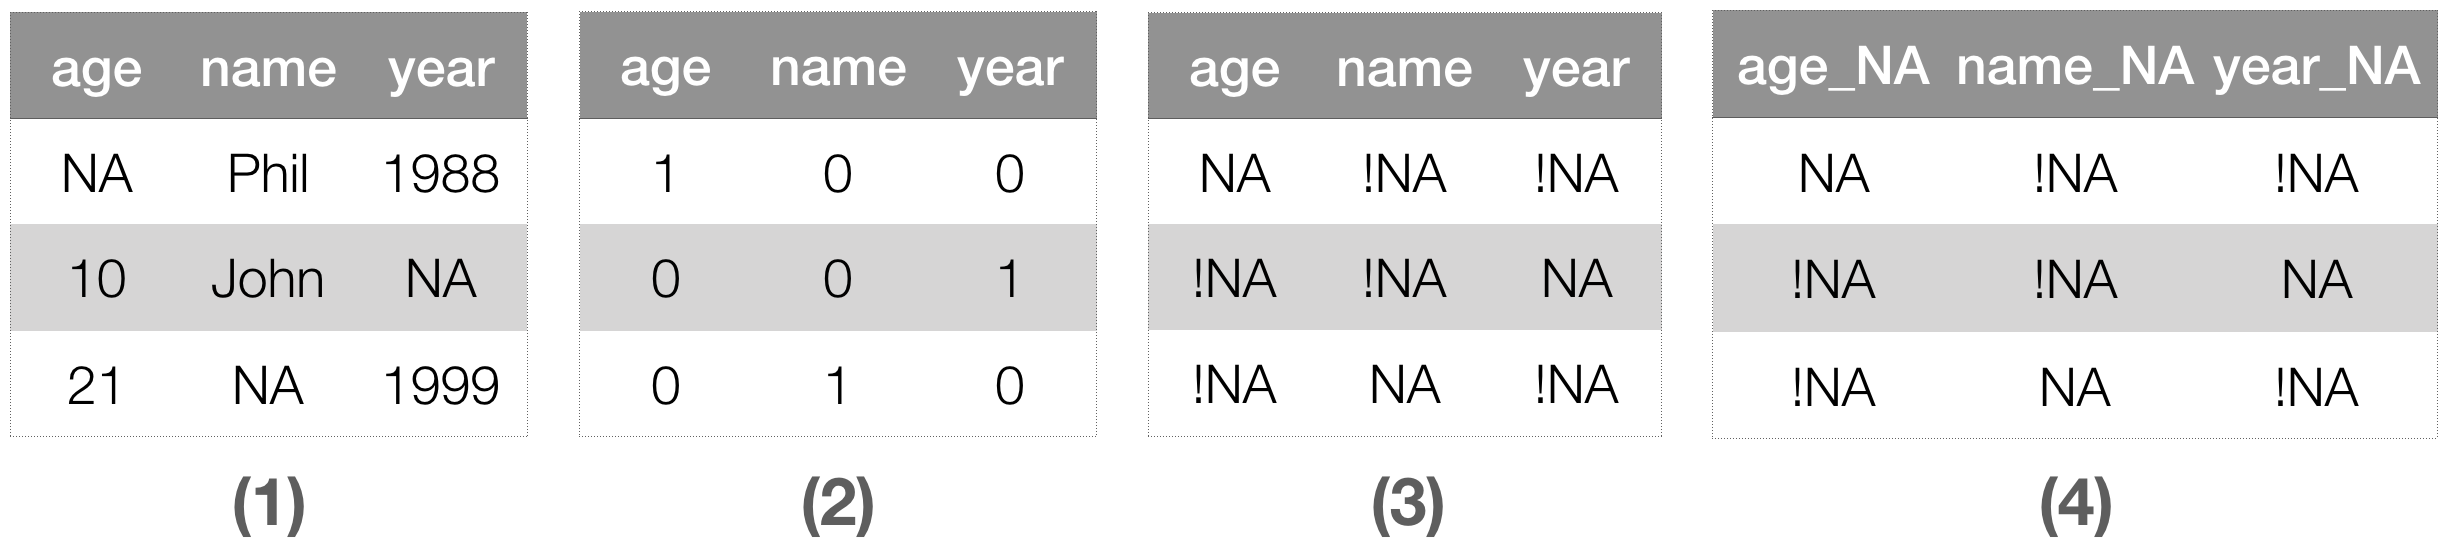
\includegraphics[width=1\linewidth]{full-conversion-to-shadow} 

}

\caption{Progression of creating shadow matrix data. (1-2) Data to a binary representation of missings, (2-3) Binary format converted to a shadow matrix (3-4) New and improved shadow matrix with changed variable names. This clearly links a variable to its state of missingness.}\label{fig:shadow-matrix-progress}
\end{figure}

Three features are added to the shadow matrix to facilitate analysis:

\begin{enumerate}
\def\labelenumi{\arabic{enumi}.}
\item
  Coordinated names: Variables in the shadow matrix gain the same name
  as in the data, with the suffix "\_NA".
\item
  Special missing values: Values in the shadow matrix can be ``special''
  missing values, indicated as \texttt{NA\_suffix}, where ``suffix'' is
  a very short message of the type of missings.
\item
  Cohesiveness: Binding the shadow matrix column-wise to the original
  data creates a cohesive \emph{nabular} data form, useful for
  visualization and summaries.
\end{enumerate}

These additions are now discussed in turn.

\hypertarget{coordinated-names}{%
\subsubsection{Coordinated names}\label{coordinated-names}}

A consistent short suffix ``\texttt{\_NA}'' for each variable keeps
names coordinated throughout analysis (See Figure
\ref{fig:shadow-matrix-progress} part 4). The suffix is short and easy
to remember in analysis or visualization. It also makes a clear
distinction that \texttt{var\_NA} is a random variable of the
missingness of a variable, \texttt{var}. This subtle change is important
as it changes the focus from the value of a variable to it's missingness
state, making intent clear when performing analysis.

\hypertarget{special-missings}{%
\subsubsection{Special missings}\label{special-missings}}

Values in the shadow matrix are ``factor'' type values, with text values
``NA'' and ``!NA'' and underlying number values 1 and 0, for missing and
not missing. Extending these to include ``special'' missing values
labelled as ``NA\_\textless{}suffix\textgreater{}'' allows for
representing additional features such as instrument failure and drop-out
as ``NA\_instr\_fail'', and ``NA\_drop\_out''. The underlying number
representation changes from binary to integer. For example, instrument
failure and drop out would be represented as 2 and 3, see Table
\ref{tab:shadow-encoding} for an example. Encoding these special missing
values is achieved by defining logical conditions and suffixes with the
\texttt{recode\_shadow} function in \texttt{naniar}, shown in Section
\ref{verbs-recode}.

\begin{table}[!h]

\caption{\label{tab:shadow-encoding}Example data of temperature, and its observed value, shadow representation, and underlying value. The temperature value of -99 is represented in the shadow column as 'NA\_instr', which in turn has the underlying numeric value of 2. This captures additional information about the data that is otherwise difficult to record.}
\centering
\begin{tabular}[t]{rlr}
\toprule
temp & temp\_NA & NA\_value\\
\midrule
-99 & NA\_instr & 2\\
NA & NA & 1\\
-1 & NA\_dropout & 3\\
106 & !NA & 0\\
\bottomrule
\end{tabular}
\end{table}

\hypertarget{nabular-data}{%
\subsubsection{Nabular data}\label{nabular-data}}

\emph{Nabular} data binds the shadow matrix column-wise to the original
data, and is so named as a portmanteau of \texttt{NA} and
\texttt{tabular}. \emph{Nabular} data keeps corresponding rows together,
removing the possibility of mismatching records, and explicitly links
missing values to the data. \emph{Nabular} data facilitates
visualization and summaries by allowing the user to reference the
missingness of a variable, \texttt{var}, as \texttt{var\_NA}.
\emph{Nabular} data is a snapshot of the missingness of the data. This
means when \emph{nabular} data is imputed, those imputed values can
easily be identified in analysis by referring to the appropriate,
coordinated names. \emph{Nabular} data is created using the command
\texttt{bind\_shadow()} or \texttt{nabular()} (see Figure
\ref{fig:nabularfig}). \emph{Nabular} data is not unlike classical data
formats that have quality or flag columns associated with each measured
variable, e.g.~Scripps CO2 data (Keeling et al. 2005), GHCN data (Durre
et al. 2008).

\begin{figure}

{\centering 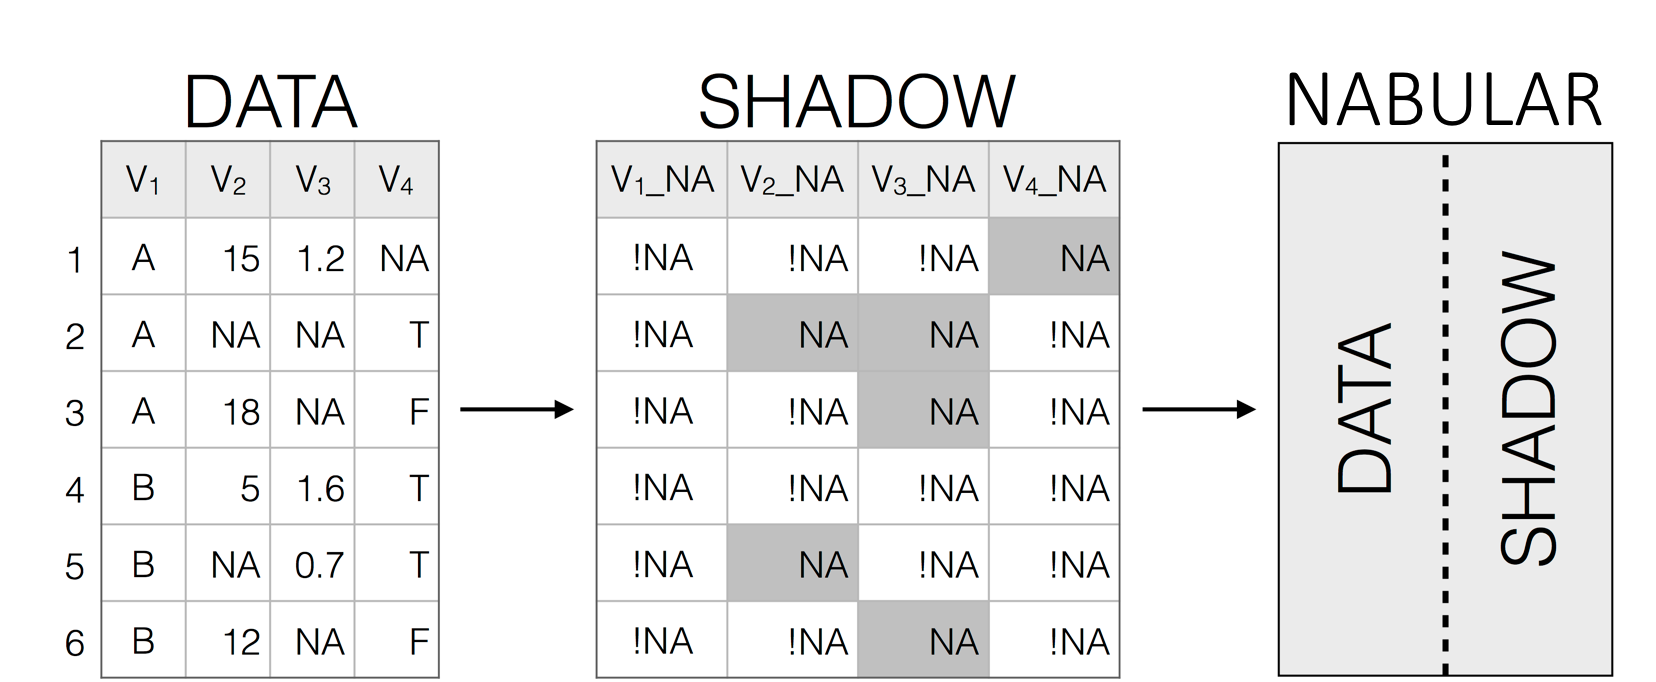
\includegraphics[width=1\linewidth]{nabular} 

}

\caption{The process of creating nabular data. Data transformed to shadow matrix, and nabular data contains the shadow matrix, column bound to the data. Nabular data can be created using `bind\_shadow` or `nabular()` functions. Nabular data provides a useful format for missing data exploration and analysis.}\label{fig:nabularfig}
\end{figure}

A data structure for missing data provides key benefits over on-the-fly
creating a logical matrix where TRUE means missing, and FALSE means
present. Firstly, it can be confusing to users whether TRUE or FALSE
means missing or present; \texttt{NA} and \texttt{!NA} are clearer.
Secondly, special missing values cannot be added fluently during
analysis with a logical matrix. Finally, the logical matrix cannot
capture which values are imputed, if imputation has already taken place.
Imputing values on \emph{nabular} data automatically tracks these value
changes.

Using additional columns to represent missingness information follows
recently published best practices for data organization, described in
Ellis and Leek (2017) and Broman and Woo (2017): (1) Keep one thing in a
cell and (2) Describe additional features of variables in a second
column. Here they suggest to indicate censored data with an extra
variable called ``VariableNameCensored'', which would be TRUE if
censored, otherwise FALSE. This information is now represented in the
shadow columns as additional integers, along with the other missing
information.

Other statistical programs represent missingness values as a full-stop,
\texttt{.}, and allow for recording special missing values as
\texttt{.a} through to \texttt{.z}. The special values from these
languages break the rule of ``keeping one thing in a cell'', as they
record both the value and the multivariate missingness state.

\hypertarget{vis-summaries}{%
\subsection{Visual summaries}\label{vis-summaries}}

Visualizing missingness in a dataset is essential to understand its
structure. This section discusses visualizations that are easy to
remember and compose with other functions in a pipeline. Four different
areas of visualization of missing data are discussed: overviews (Section
\ref{overview-plots}); univariate (Section \ref{univariate-plots}),
bivariate (Section \ref{bivariate-plots}), and multivariate (Section
\ref{multivariate-plots}). All plots are created using \texttt{ggplot2},
giving users clearer control over the plot appearance, and
customizability.

\hypertarget{overview-plots}{%
\subsubsection{Overview plots}\label{overview-plots}}

The number of missings in each variable and case are visualized using
\texttt{gg\_miss\_var} and \texttt{gg\_miss\_case} (see Figure
\ref{fig:gg-miss-case-var} below). These are shown using the
``airquality'' dataset, included in base R, which contains daily air
quality measurements in New York, from May to September, 1973. Rather
than highlighting the amount of complete data, these visualizations draw
attention to the amount of missings, ordering by missingness.

\begin{figure}

{\centering 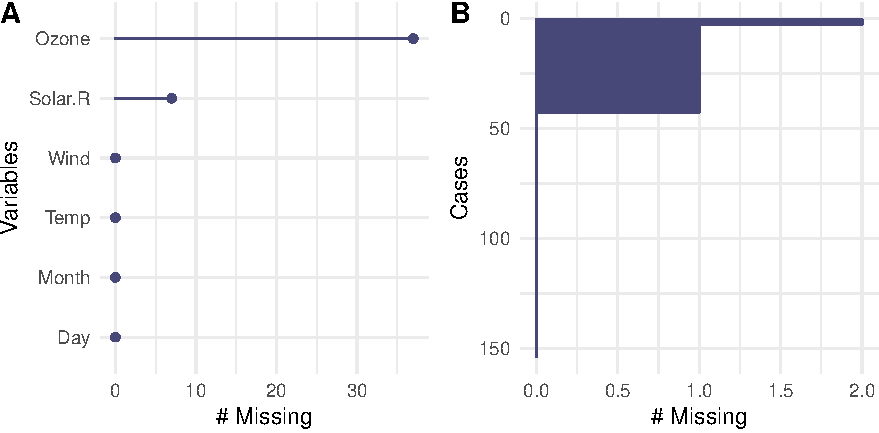
\includegraphics[width=0.9\linewidth]{tidy-missing-data-paper_files/figure-latex/gg-miss-case-var-1} 

}

\caption{Graphical summaries of missingness in variables and cases for the airquality data. (A) Missings in each variable and (B) in each case. There are missing values in Ozone and Solar.R, with Ozone having more missings, and not many cases have two missing values, with most missingness being from cases with one missing value.}\label{fig:gg-miss-case-var}
\end{figure}

All missings in a dataset can be displayed using a heatmap style
visualization. This is achieved using \texttt{vis\_miss()} from the
\texttt{visdat} package (Tierney 2017), which also provides summaries of
missingness overall in the legend, and for each column (see Figure
\ref{fig:vis-miss}). The user can also apply clustering to the rows, and
arrange columns by missingness (Figure \ref{fig:vis-miss}B). Similar
visualizations are available in other missing data packages such as
\texttt{VIM}, \texttt{mi}, \texttt{Amelia}, and \texttt{MissingDataGUI}.
A key improvement is that \texttt{vis\_miss()} orients the visualization
analogous to a regular data structure: variables form columns in the
visualization and are named at the top, and each row is an observation.
Using \texttt{ggplot2} means the plot can be customized and combined
with other ggplot graphics.

\begin{figure}

{\centering 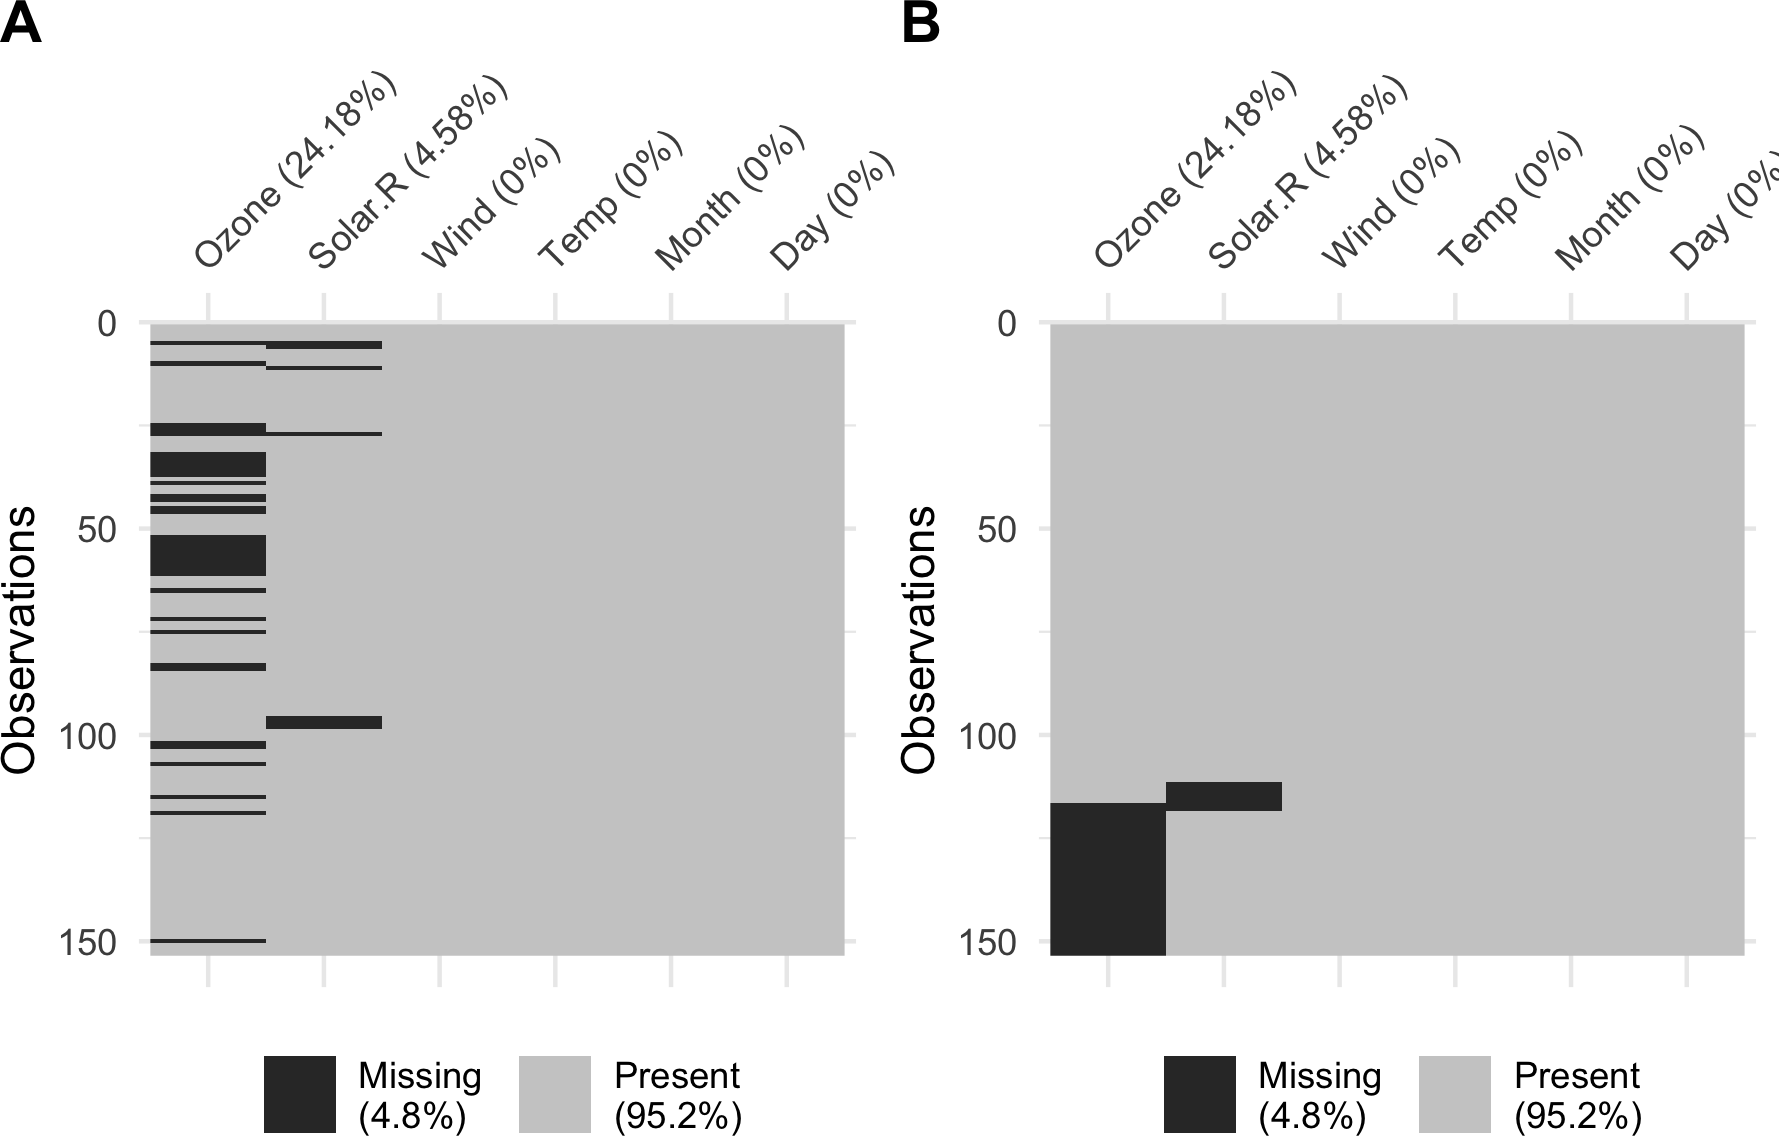
\includegraphics[width=0.95\linewidth]{tidy-missing-data-paper_files/figure-latex/vis-miss-1} 

}

\caption{Heatmap visualizations of missing data for the airquality dataset. (A) The default output and (B) ordered by clustering on rows and columns. There are only missings in ozone and solar radiation, and there appears to be some structure to their missingness.}\label{fig:vis-miss}
\end{figure}

The number of times certain variables go missing together can be
visualized using an ``upset plot'' (Conway et al. 2017), a visualization
technique for showing the size and features of sets in data that is
similar to a venn diagram, but scales better with more variables (Figure
\ref{fig:airquality-upset}).

\begin{figure}

{\centering 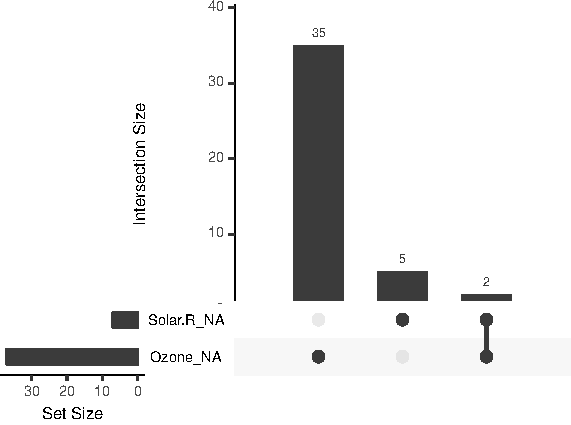
\includegraphics[width=0.8\linewidth]{tidy-missing-data-paper_files/figure-latex/airquality-upset-1} 

}

\caption{The pattern of missingness in the airquality dataset shown in an upset plot. Only Ozone and Solar.R have missing values, and Ozone has the most missing values. There are 2 cases where both Solar.R and Ozone have missing values.}\label{fig:airquality-upset}
\end{figure}

Figure \ref{fig:airquality-upset} shows that only Ozone and Solar.R have
missing values. The dots in the bottom right show the combinations of
missingness, with the bottom left showing the missingness in each
variable, and the top showing the missingness for the combinations. The
bottom left shows that Ozone has the most missing values, and the top
shows 2 cases where both Solar.R and Ozone have missing values together.

\hypertarget{univariate-plots}{%
\subsubsection{Univariate plots}\label{univariate-plots}}

Missing values are by default not shown for univariate visualizations
such as histograms or densities. Two ways to use \emph{nabular} data to
present univariate data with missings are discussed. The first imputes
values below the range to facilitate visualizations. The second displays
two plots of the same variable according to the missingness of a chosen
variable.

\hypertarget{imp-below-range}{%
\paragraph{Imputing values below the range}\label{imp-below-range}}

To visualize the amount of missings in each variable, the data is
transformed into \emph{nabular} form, then values are imputed values
below the range of data using \texttt{impute\_below} (by default
imputing 10\% below the range). Visualizing this as a histogram shows
missing values on its left. Ozone is shown in a different color by
referring to the variable \texttt{Ozone} as \texttt{Ozone\_NA} in a fill
aesthetic in ggplot, shown in Figure \ref{fig:impute-shift-histogram}.

\begin{figure}

{\centering 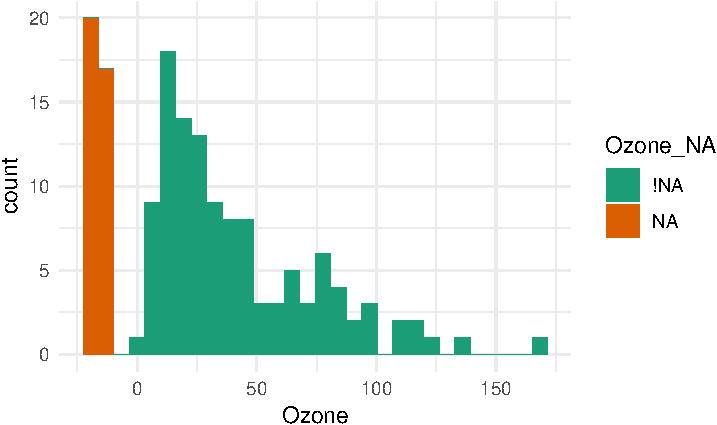
\includegraphics[width=0.75\linewidth]{tidy-missing-data-paper_files/figure-latex/impute-shift-histogram-1} 

}

\caption{A histogram using nabular data to show the values and missings in ozone. Values are imputed below the range to show the number of missings in Ozone and colored according to missingness of ozone (`Ozone\_NA`). There are about 35 missings in Ozone.}\label{fig:impute-shift-histogram}
\end{figure}

\hypertarget{vis-split-by-miss}{%
\paragraph{Univariate split by missingness}\label{vis-split-by-miss}}

Missingness of one variable can also be used to display different
distributions in another. Figure \ref{fig:bind-shadow-density} shows the
values of temperature when ozone is present, and missing. Figure
\ref{fig:bind-shadow-density}A is a faceted histogram, and Figure
\ref{fig:bind-shadow-density}B is an overlaid density. This shows how
values of temperature are affected by the missingness of ozone, and
reveals a cluster of low temperature observations with missing ozone
values.

\begin{figure}

{\centering 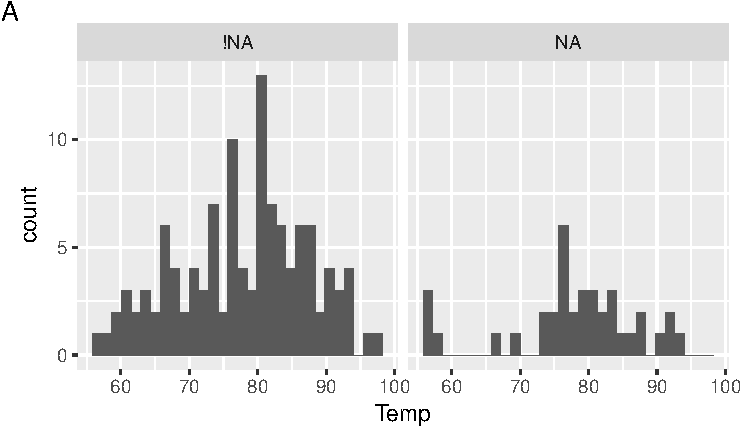
\includegraphics[width=0.49\linewidth]{tidy-missing-data-paper_files/figure-latex/bind-shadow-density-1} 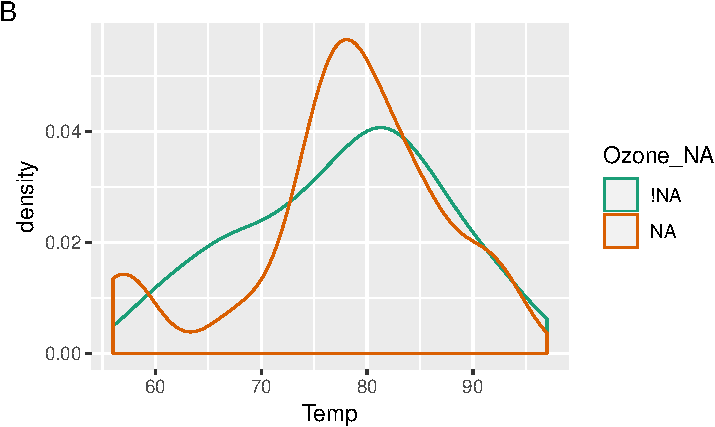
\includegraphics[width=0.49\linewidth]{tidy-missing-data-paper_files/figure-latex/bind-shadow-density-2} 

}

\caption{A visualization of temperature according to missingness in ozone from in the airquality dataset. A histogram of temperature facetted by the missingness of ozone (A), or a density of temperature colored by missingness in ozone (B). The distribution shows a cluster of low temperature observations with missing ozone values, but the temperature values are otherwise similar.}\label{fig:bind-shadow-density}
\end{figure}

\hypertarget{bivariate-plots}{%
\subsubsection{Bivariate plots}\label{bivariate-plots}}

To visualize missing values in two dimensions the missing values can be
placed in the plot margins. This is achieved by imputing values below
the range of the data. As in Section \ref{imp-below-range}, using
\emph{nabular} data identifies imputed values, and color makes
missingness pre-attentive (Treisman 1985). The steps of imputing and
coloring have been been combined into \texttt{geom\_miss\_point()} from
the \texttt{naniar} package (Figure \ref{fig:geom-miss}), where there is
a mostly uniform spread of missing values for Solar.R and Ozone.

\begin{figure}

{\centering 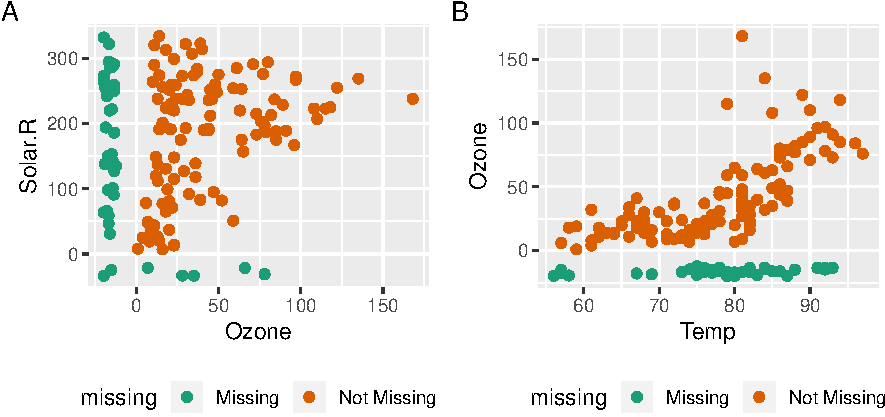
\includegraphics{tidy-missing-data-paper_files/figure-latex/geom-miss-1} 

}

\caption{Scatterplots with missings displayed at 10 percent below for the airquality dataset. Scatterplots of ozone and solar radiation (A), and ozone and temperature (B). There are missings in ozone and solar radiation, but not temperature.}\label{fig:geom-miss}
\end{figure}

As \texttt{geom\_miss\_point} is a defined geometry for
\texttt{ggplot2}, it provides features such as faceting and mapping
other variables to aesthetics such as color, shape, or size. The shadow
format by itself can also be used to visually explore some patterns of
missingness.

\hypertarget{multivariate-plots}{%
\subsubsection{Multivariate plots}\label{multivariate-plots}}

Parallel coordinate plots can visualize missingness beyond two
dimensions. They transform variables to the same scale, and typically
make the data values range between 0 and 1. To showcase this
visualization, the dataset \texttt{oceanbuoys} from \texttt{naniar} is
used, which contains measurements of moored ocean buoys to understand
and predict El Niño and El Niña. The data were collected in 1993 and
1997, and contains information on the sea and air temperature, humidity,
and east west and north south wind directions.

Figure \ref{fig:parallel-cord-plot} shows a parallel coordinate plot of
the \texttt{oceanbuoys} data, with missing values imputed to be 10\%
below the range, and values colored according to whether humidity
contained missing values. Although a 10\% below imputation is not the
most ideal way to display missing values in a parallel coordinate plot,
it shows that humidity is missing at low air and sea temperatures, and
that humidity is missing in one year, and one location.

\begin{figure}

{\centering 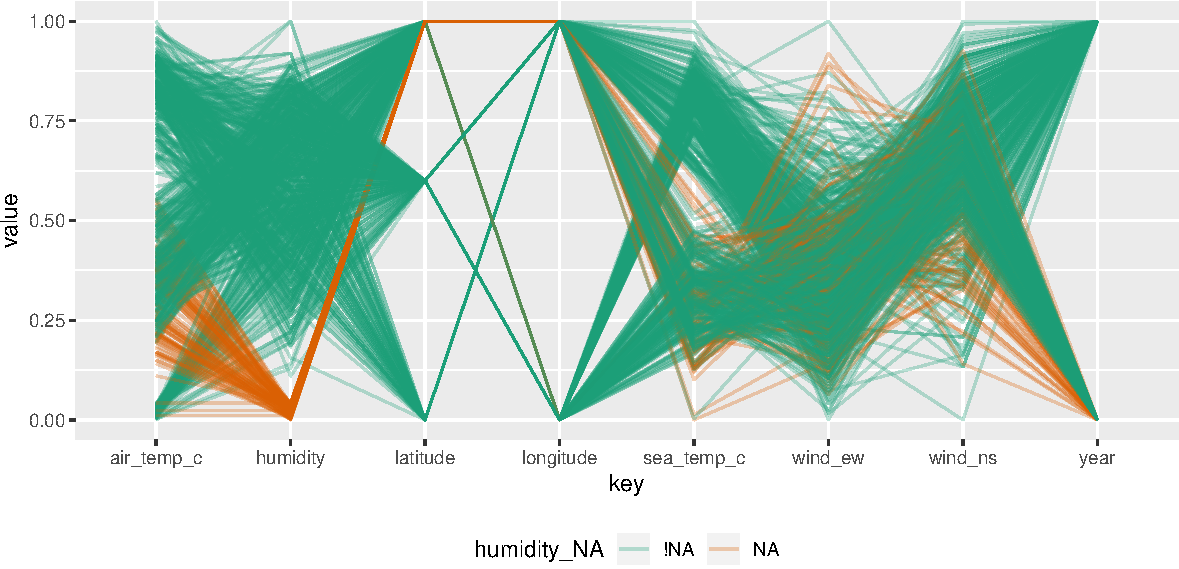
\includegraphics[width=1\linewidth]{tidy-missing-data-paper_files/figure-latex/parallel-cord-plot-1} 

}

\caption{Parallel coordinate plot shows missing values imputed 10\% below range for the oceanbuoys dataset. Values are colored by missingness of humidity. Humidity is missing for low air and sea temperatures, and is missing for one year and one location. }\label{fig:parallel-cord-plot}
\end{figure}

\hypertarget{num-sum}{%
\subsection{Numerical summaries}\label{num-sum}}

There are different ways to summarize the amount of missing and complete
values in a dataset. This section describes approaches to summarizing
missingness, implemented in the \texttt{naniar} package. The functions
are easy to remember as they follow consistent naming, and their output
is consistent, and returns a single number or dataframe. This means they
integrate well with plotting and modelling tools. Section
\ref{single-num-sum} discusses single number summaries for all data and
for cases and variables ; Section \ref{sum-tab-missings} discusses
variable- and case-wise summaries; and Section \ref{num-sum-w-group}
shows how the design of these tools works with other tools in an
analysis pipeline.

\hypertarget{single-num-sum}{%
\subsubsection{Single number summaries}\label{single-num-sum}}

The overall number of missing values in a dataset is shown with
\texttt{n\_miss}, and the proportion or percent missings,
\texttt{prop\_miss} and \texttt{pct\_miss}. Complementing these are
functions to reveal the number of complete values: \texttt{n\_complete},
\texttt{prop\_complete}, and \texttt{pct\_complete}. These be extended
to summarize the number/amount of variables and cases that contain a
missing values by appending \texttt{\_case} or \texttt{\_var} to any of
these summaries. Table \ref{tab:n-prop-pct-miss-complete} shows the
names and output of these functions on the dataset airquality.

\begin{table}[!h]

\caption{\label{tab:n-prop-pct-miss-complete}Single number summaries of missing and complete data, applied to the airquality dataset. These functions follow consistent naming, to make them easy to remember, and to make their use clear.}
\centering
\begin{tabular}[t]{lrlr}
\toprule
Missing Function & missing value & Complete function & complete value\\
\midrule
n\_miss & 44.00 & n\_complete & 874.00\\
prop\_miss & 0.05 & prop\_complete & 0.95\\
pct\_miss & 4.79 & pct\_complete & 95.21\\
pct\_miss\_var & 27.45 & prop\_complete\_var & 0.73\\
pct\_miss\_case & 33.33 & pct\_complete\_case & 66.67\\
\bottomrule
\end{tabular}
\end{table}

\hypertarget{sum-tab-missings}{%
\subsubsection{Summaries and tabulations of missing
data}\label{sum-tab-missings}}

Presenting the number and percent of missing values for each variable,
or case, provides a summary that can be used by models to inform
imputations or data handling. For example, potentially dropping
variables or deciding to include others in an imputation model. Another
useful approach is to tabulate the frequency of missing values for each
variable or case; that is, the number of times there are zero, one, two,
and so on, missing values. These summaries and tabulations are shown for
variable in Tables \ref{tab:miss-var-summary} and
\ref{tab:miss-var-table}, using the \texttt{miss\_var\_summary} and
\texttt{miss\_var\_table} functions. Functions are also provided for
case-wise summaries and tabulations with \texttt{miss\_case\_summary}
and \texttt{miss\_case\_table}, which order by \texttt{n\_miss}, so the
most missings are always shown at the top. Other summaries provided in
\texttt{naniar} include summaries of missingness across a provided
repeating span, \texttt{miss\_var\_span}, and finding the streaks or
runs of missingness in a given variable in \texttt{miss\_var\_run}.

\begin{table}[!h]

\caption{\label{tab:miss-var-summary}Summary of the number and percent of missings in each variable. Only ozone and solar radiation have missing values.}
\centering
\begin{tabular}[t]{lrr}
\toprule
variable & n\_miss & pct\_miss\\
\midrule
Ozone & 37 & 24.2\\
Solar.R & 7 & 4.6\\
Wind & 0 & 0.0\\
Temp & 0 & 0.0\\
Month & 0 & 0.0\\
Day & 0 & 0.0\\
\bottomrule
\end{tabular}
\end{table}

\begin{table}[!h]

\caption{\label{tab:miss-var-table}Tabulation of the amount of missing data in each variable. This shows the number of variables with no missings, 7 missings, and 37 missings, and the percentage of variables with those amounts of missingness. There are not many patterns of missingness.}
\centering
\begin{tabular}[t]{rrr}
\toprule
n\_miss\_in\_var & n\_vars & pct\_vars\\
\midrule
0 & 4 & 66.7\\
7 & 1 & 16.7\\
37 & 1 & 16.7\\
\bottomrule
\end{tabular}
\end{table}

\hypertarget{num-sum-w-group}{%
\subsubsection{Combining numerical summaries with grouping
operations}\label{num-sum-w-group}}

These summaries and tabulations can be composed with the ``pipe''
operator to perform grouped summaries using the \texttt{group\_by}
operator from \texttt{dplyr}. These summaries return dataframes, which
may be used by other plotting devices, modelling tools, or other
summaries. Table \ref{tab:group-miss-var-summary} shows an example of
the missing data summaries for the airquality dataset in each variable,
for each month of the year. These datasets can be summarized in
visualizations, or values input into a model.

\begin{table}[!h]

\caption{\label{tab:group-miss-var-summary}A summary of the missingness in each variable, for each Month of the airquality dataset, with only the first 10 rows of output shown. There are more ozone missings in June than May.}
\centering
\begin{tabular}[t]{rlrr}
\toprule
Month & variable & n\_miss & pct\_miss\\
\midrule
5 & Ozone & 5 & 16.1\\
5 & Solar.R & 4 & 12.9\\
5 & Wind & 0 & 0.0\\
5 & Temp & 0 & 0.0\\
5 & Day & 0 & 0.0\\
\addlinespace
6 & Ozone & 21 & 70.0\\
6 & Solar.R & 0 & 0.0\\
6 & Wind & 0 & 0.0\\
6 & Temp & 0 & 0.0\\
6 & Day & 0 & 0.0\\
\bottomrule
\end{tabular}
\end{table}

\hypertarget{verbs}{%
\subsection{Verbs}\label{verbs}}

Common operations on missing data can be considered to be verbs: scan,
replace, add, shadow, impute, track, and flag. Missing values can be
\textbf{scanned} to find possible missings not coded as \texttt{NA}.
These values can then be \textbf{replaced} with an \texttt{NA} value. To
facilitate exploration, summaries of missingness can be \textbf{added}
as a summary column to the original data. Data values can be augmented
with \textbf{shadow} values, which helps explore missing data, as well
as facilitating the process of \textbf{imputing}, and \textbf{tracking}.
Finally, unusual or specially coded missing values can be
\textbf{flagged}. These verbs are described in this section.

\hypertarget{verbs-search}{%
\subsubsection{scan: Searching for common missing value
labels}\label{verbs-search}}

There are many common values that mean ``missing''. For example, ``N/A''
``Not Available'', ``MISSING'', or white space " ". Before replacing
these values with missing values (\texttt{NA}), it is useful to first
\emph{scan} the data to get a sense of the magnitude of the problem. The
\texttt{miss\_scan\_count()} function finds where specified values occur
in data. For example, for the example data, \texttt{dat\_ms}:

\begin{table}[!h]

\caption{\label{tab:setup-miss-scan-count}An example dataset with variables x, y and z containing some common unusual missing values.}
\centering
\begin{tabular}[t]{rlr}
\toprule
x & y & z\\
\midrule
1 & A & -100\\
3 & N/A & -99\\
NA & NA & -98\\
-99 & E & -101\\
-98 & F & -1\\
\bottomrule
\end{tabular}
\end{table}

All occurrences of -99 can be searched for using the code:

\begin{Shaded}
\begin{Highlighting}[]
\KeywordTok{miss_scan_count}\NormalTok{(}\DataTypeTok{data =}\NormalTok{ dat_ms, }\DataTypeTok{search =} \DecValTok{-99}\NormalTok{)}
\end{Highlighting}
\end{Shaded}

This returns a table of the occurrences of that value in each variable
(Table \ref{tab:miss-scan-count}). A list of common NA values is
provided in \texttt{naniar} in the \texttt{common\_na\_strings} and
\texttt{common\_na\_numbers} for characters and numbers. These contain
values like ``n/a'', ``na'', and ``.'', and -9, -99.

\begin{table}[!h]

\caption{\label{tab:miss-scan-count}Table of the occurences of the search '-99' in the data, 'dat\_ms'. There is one occurence if -99 in variables x and z.}
\centering
\begin{tabular}[t]{lr}
\toprule
Variable & n\\
\midrule
x & 1\\
y & 0\\
z & 1\\
\bottomrule
\end{tabular}
\end{table}

\hypertarget{verbs-replace-with}{%
\subsubsection{replace: Replacing missing value label with
another}\label{verbs-replace-with}}

Once the magnitude of the unusual missing values has been assessed,
these values need to be replaced with appropriate missing values, using
\texttt{replace\_with\_na}. This is useful when there is certainty of
which values mean missing. For example ``N/A'', ``N A'', ``Not
Available'', and ``missing''. Using the previous toy dataset,
\texttt{dat\_ms}, the value -99, or both -99 and 98 can be replaced with
NA as follows:

\begin{Shaded}
\begin{Highlighting}[]
\KeywordTok{replace_with_na}\NormalTok{(dat_ms, }\DataTypeTok{replace =} \KeywordTok{list}\NormalTok{(}\DataTypeTok{x =} \DecValTok{-99}\NormalTok{))}
\end{Highlighting}
\end{Shaded}

\begin{verbatim}
## # A tibble: 5 x 3
##       x y         z
##   <dbl> <chr> <dbl>
## 1     1 A      -100
## 2     3 N/A     -99
## 3    NA <NA>    -98
## 4    NA E      -101
## 5   -98 F        -1
\end{verbatim}

\begin{Shaded}
\begin{Highlighting}[]
\KeywordTok{replace_with_na}\NormalTok{(dat_ms, }\DataTypeTok{replace =} \KeywordTok{list}\NormalTok{(}\DataTypeTok{x =} \KeywordTok{c}\NormalTok{(}\OperatorTok{-}\DecValTok{99}\NormalTok{, }\DecValTok{-98}\NormalTok{)))}
\end{Highlighting}
\end{Shaded}

\begin{verbatim}
## # A tibble: 5 x 3
##       x y         z
##   <dbl> <chr> <dbl>
## 1     1 A      -100
## 2     3 N/A     -99
## 3    NA <NA>    -98
## 4    NA E      -101
## 5    NA F        -1
\end{verbatim}

For flexibility, there are scoped variants for
\texttt{replace\_with\_na}: \texttt{\_all}, \texttt{\_if}, and
\texttt{\_at}. This means \texttt{replace\_with\_na} works for
\textbf{all} variables with \texttt{replace\_with\_na\_all}, \textbf{at}
selected variables with \texttt{replace\_with\_na\_at}, and \textbf{if}
variables that meet some condition with \texttt{replace\_with\_na\_if}.
The syntax for these is slightly different to
\texttt{replace\_with\_na}, but powerful:

\begin{Shaded}
\begin{Highlighting}[]
\KeywordTok{replace_with_na_at}\NormalTok{(}\DataTypeTok{data =}\NormalTok{ dat_ms,}
                   \DataTypeTok{.vars =} \StringTok{"x"}\NormalTok{,}
                   \DataTypeTok{condition =} \OperatorTok{~}\NormalTok{.x }\OperatorTok{==}\StringTok{ }\DecValTok{-99}\NormalTok{)}
\end{Highlighting}
\end{Shaded}

\begin{verbatim}
## # A tibble: 5 x 3
##       x y         z
##   <dbl> <chr> <dbl>
## 1     1 A      -100
## 2     3 N/A     -99
## 3    NA <NA>    -98
## 4    NA E      -101
## 5   -98 F        -1
\end{verbatim}

\begin{Shaded}
\begin{Highlighting}[]
\KeywordTok{replace_with_na_if}\NormalTok{(}\DataTypeTok{data =}\NormalTok{ dat_ms,}
                 \DataTypeTok{.predicate =}\NormalTok{ is.character,}
                 \DataTypeTok{condition =} \OperatorTok{~}\NormalTok{.x }\OperatorTok{==}\StringTok{ "N/A"}\NormalTok{)}
\end{Highlighting}
\end{Shaded}

\begin{verbatim}
## # A tibble: 5 x 3
##       x y         z
##   <dbl> <chr> <dbl>
## 1     1 A      -100
## 2     3 <NA>    -99
## 3    NA <NA>    -98
## 4   -99 E      -101
## 5   -98 F        -1
\end{verbatim}

\begin{Shaded}
\begin{Highlighting}[]
\KeywordTok{replace_with_na_all}\NormalTok{(}\DataTypeTok{data =}\NormalTok{ dat_ms,}
                    \DataTypeTok{condition =} \OperatorTok{~}\NormalTok{.x }\OperatorTok{==}\StringTok{ }\DecValTok{-99}\NormalTok{)}
\end{Highlighting}
\end{Shaded}

\begin{verbatim}
## # A tibble: 5 x 3
##       x y         z
##   <dbl> <chr> <dbl>
## 1     1 A      -100
## 2     3 N/A      NA
## 3    NA <NA>    -98
## 4    NA E      -101
## 5   -98 F        -1
\end{verbatim}

\hypertarget{verbs-add-cols}{%
\subsubsection{add: Adding missingness summary
variables}\label{verbs-add-cols}}

Summary information such as the number of missings in a given case can
be useful in understanding missingness structure, and even more so when
this information is kept alongside the data. Functions starting with
\texttt{add\_} exist in \texttt{dplyr} to add count information for
particular groups or conditions to the data. Similarly, \texttt{naniar}
includes \texttt{add\_} functions to add missingness summary information
back to the data, such as the number or proportion of missingness, the
missingness cluster, or if there are any missings, using:
\texttt{add\_n\_miss()} \texttt{add\_prop\_miss()},
\texttt{add\_miss\_cluster}, and \texttt{add\_any\_miss()},
respectively.

An example use of these features is in Tierney et al. (2015), where the
proportion, number, or cluster of missings is used as the outcome in a
model. The variables in the dataset can then be used to predict the
outcome, identifying variables and values important in predicting
missingness structures. There are also functions for adding information
about shadow values or nice labels for if there are any missing values
with \texttt{add\_label\_shadow()} and \texttt{add\_label\_missings()}:

\begin{Shaded}
\begin{Highlighting}[]
\KeywordTok{add_n_miss}\NormalTok{(dat_ms)}
\end{Highlighting}
\end{Shaded}

\begin{verbatim}
## # A tibble: 5 x 4
##       x y         z n_miss_all
##   <dbl> <chr> <dbl>      <int>
## 1     1 A      -100          0
## 2     3 N/A     -99          0
## 3    NA <NA>    -98          2
## 4   -99 E      -101          0
## 5   -98 F        -1          0
\end{verbatim}

\begin{Shaded}
\begin{Highlighting}[]
\KeywordTok{add_prop_miss}\NormalTok{(dat_ms)}
\end{Highlighting}
\end{Shaded}

\begin{verbatim}
## # A tibble: 5 x 4
##       x y         z prop_miss_all
##   <dbl> <chr> <dbl>         <dbl>
## 1     1 A      -100         0    
## 2     3 N/A     -99         0    
## 3    NA <NA>    -98         0.667
## 4   -99 E      -101         0    
## 5   -98 F        -1         0
\end{verbatim}

\begin{Shaded}
\begin{Highlighting}[]
\KeywordTok{add_miss_cluster}\NormalTok{(dat_ms)}
\end{Highlighting}
\end{Shaded}

\begin{verbatim}
## # A tibble: 5 x 4
##       x y         z miss_cluster
##   <dbl> <chr> <dbl>        <int>
## 1     1 A      -100            1
## 2     3 N/A     -99            1
## 3    NA <NA>    -98            2
## 4   -99 E      -101            1
## 5   -98 F        -1            1
\end{verbatim}

\hypertarget{verbs-nabular}{%
\subsubsection{\texorpdfstring{shadow: Creating \texttt{nabular}
data}{shadow: Creating nabular data}}\label{verbs-nabular}}

\emph{Nabular} data has the shadow matrix column-bound to the existing
data. This facilitates visualization and summaries, and allows for
imputed values to be appropriately tracked. \emph{Nabular} data can be
created with \texttt{bind\_shadow()} or \texttt{nabular()}. The
\texttt{bind\_shadow()} function is so named to borrow from existing
functions named \texttt{bind} - such as \texttt{bind\_rows()} and
\texttt{bind\_cols()} from \texttt{dplyr}, which bind rows or columns
into a dataframe. An example use of \texttt{bind\_shadow()} on the
example data, \texttt{dat\_ms} is shown below:

\begin{Shaded}
\begin{Highlighting}[]
\KeywordTok{bind_shadow}\NormalTok{(dat_ms)}
\end{Highlighting}
\end{Shaded}

\begin{verbatim}
## # A tibble: 5 x 6
##       x y         z x_NA  y_NA  z_NA 
##   <dbl> <chr> <dbl> <fct> <fct> <fct>
## 1     1 A      -100 !NA   !NA   !NA  
## 2     3 N/A     -99 !NA   !NA   !NA  
## 3    NA <NA>    -98 NA    NA    !NA  
## 4   -99 E      -101 !NA   !NA   !NA  
## 5   -98 F        -1 !NA   !NA   !NA
\end{verbatim}

\hypertarget{verbs-recode}{%
\subsubsection{flag: Describing different types of missing
values}\label{verbs-recode}}

Unusual or spurious data values are often identified and
\texttt{flagged}. For example, there might be special codes to mark an
individual dropping out of a study, known instrument failure in weather
instruments, or for values censored in analysis. These special types of
missingness can be encoded in the shadow matrix of \emph{nabular} data,
using the \texttt{recode\_shadow()} function. This provides a fluent
interface to recode, or flag, the shadow information in the shadow
matrix as a special type of missing value. Using
\texttt{recode\_shadow()} requires specifying the variable you want to
contain the flagged value, the condition you want this to occur at, and
a suffix for the new type of missing value. This is then recoded as a
new factor level in the shadow matrix, so that every column is aware of
all possible new values of missingness. For example, the values -99 and
-98 could be recoded to mean a broken machine sensor for the variable x:

\begin{Shaded}
\begin{Highlighting}[]
\NormalTok{dat_ms }\OperatorTok
\StringTok{  }\KeywordTok{bind_shadow}\NormalTok{() }\OperatorTok
\StringTok{  }\KeywordTok{recode_shadow}\NormalTok{(}\DataTypeTok{x =} \KeywordTok{.where}\NormalTok{(x }\OperatorTok{==}\StringTok{ }\DecValTok{-99} \OperatorTok{~}\StringTok{ "broken_sensor"}\NormalTok{))}
\end{Highlighting}
\end{Shaded}

\begin{verbatim}
## # A tibble: 5 x 6
##       x y         z x_NA             y_NA  z_NA 
##   <dbl> <chr> <dbl> <fct>            <fct> <fct>
## 1     1 A      -100 !NA              !NA   !NA  
## 2     3 N/A     -99 !NA              !NA   !NA  
## 3    NA <NA>    -98 NA               NA    !NA  
## 4   -99 E      -101 NA_broken_sensor !NA   !NA  
## 5   -98 F        -1 !NA              !NA   !NA
\end{verbatim}

\hypertarget{verbs-impute}{%
\subsubsection{impute: Imputing values}\label{verbs-impute}}

\texttt{naniar} does not reinvent the wheel for imputation, as there are
many robust R packages for imputation, such as \texttt{mice},
\texttt{mi}, \texttt{VIM}, and \texttt{simputation}. However,
\texttt{naniar} does provide a few imputation methods to facilitate
exploration and visualizations, which were not otherwise available:
\texttt{impute\_below} and \texttt{impute\_mean} and
\texttt{impute\_median}. These imputation methods are useful to explore
structure in missingness, but are not recommended for use in analysis.

The \texttt{impute\_below} function imputes values below the minimum of
the data, with some jitter to reduce overplotting, but has options to
change the default amount it is shifted below, and the amount of jitter.

\begin{verbatim}
##       Ozone Solar.R
## 1  41.00000     190
## 2  36.00000     118
## 3  12.00000     149
## 4  18.00000     313
## 5 -19.72321      NA
## 6  28.00000      NA
\end{verbatim}

Similar to \texttt{simputation}, each \texttt{impute\_} function returns
the data with values imputed. However, \texttt{naniar} does not use a
formula syntax, and instead each function implements ``scoped variants''
\texttt{\_all}, \texttt{\_at} and \texttt{\_if}. Here, \texttt{\_all}
operates on \textbf{all} columns, \texttt{\_at} operates \textbf{at}
specific columns, and \texttt{\_if} operates on columns \textbf{if} they
meet some condition (such as \texttt{is.numeric} or
\texttt{is.character}). The \texttt{impute\_} functions with no scoped
variant, e.g., \texttt{impute\_mean}, will work on a single vector, but
not a data.frame. An example usage is shown below:

\begin{Shaded}
\begin{Highlighting}[]
\KeywordTok{impute_mean}\NormalTok{(airquality}\OperatorTok{$}\NormalTok{Ozone) }\OperatorTok\StringTok{ }\KeywordTok{head}\NormalTok{()}
\end{Highlighting}
\end{Shaded}

\begin{verbatim}
## [1] 41.00000 36.00000 12.00000 18.00000 42.12931 28.00000
\end{verbatim}

\begin{Shaded}
\begin{Highlighting}[]
\KeywordTok{impute_mean_at}\NormalTok{(airquality, }\DataTypeTok{.vars =} \KeywordTok{vars}\NormalTok{(Ozone)) }\OperatorTok\StringTok{ }\KeywordTok{head}\NormalTok{()}
\end{Highlighting}
\end{Shaded}

\begin{verbatim}
##      Ozone Solar.R Wind Temp Month Day
## 1 41.00000     190  7.4   67     5   1
## 2 36.00000     118  8.0   72     5   2
## 3 12.00000     149 12.6   74     5   3
## 4 18.00000     313 11.5   62     5   4
## 5 42.12931      NA 14.3   56     5   5
## 6 28.00000      NA 14.9   66     5   6
\end{verbatim}

\begin{Shaded}
\begin{Highlighting}[]
\KeywordTok{impute_mean_if}\NormalTok{(airquality, }\DataTypeTok{.predicate =}\NormalTok{ is.integer) }\OperatorTok\StringTok{ }\KeywordTok{head}\NormalTok{()}
\end{Highlighting}
\end{Shaded}

\begin{verbatim}
##      Ozone  Solar.R Wind Temp Month Day
## 1 41.00000 190.0000  7.4   67     5   1
## 2 36.00000 118.0000  8.0   72     5   2
## 3 12.00000 149.0000 12.6   74     5   3
## 4 18.00000 313.0000 11.5   62     5   4
## 5 42.12931 185.9315 14.3   56     5   5
## 6 28.00000 185.9315 14.9   66     5   6
\end{verbatim}

\begin{Shaded}
\begin{Highlighting}[]
\KeywordTok{impute_mean_all}\NormalTok{(airquality) }\OperatorTok\StringTok{ }\KeywordTok{head}\NormalTok{()}
\end{Highlighting}
\end{Shaded}

\begin{verbatim}
##      Ozone  Solar.R Wind Temp Month Day
## 1 41.00000 190.0000  7.4   67     5   1
## 2 36.00000 118.0000  8.0   72     5   2
## 3 12.00000 149.0000 12.6   74     5   3
## 4 18.00000 313.0000 11.5   62     5   4
## 5 42.12931 185.9315 14.3   56     5   5
## 6 28.00000 185.9315 14.9   66     5   6
\end{verbatim}

One drawback to imputation functions in this form is that the location
of imputed values is not tracked. This is covered in Section
\ref{verbs-track}.

\hypertarget{verbs-track}{%
\subsubsection{track: Shadow and impute missing
values}\label{verbs-track}}

To evaluate imputations they need to be tracked, which is achieved by
combining the verbs \texttt{bind\_shadow}, \texttt{impute\_}, and
\texttt{add\_label\_shadow}. The missing values can then be referred to
by their shadow variable, \texttt{\_NA}. The missingness of any
observation can be referred to with \texttt{any\_missing} (Figure
\ref{fig:track-impute-example}). The code chunk below shows the track
pattern, first using \texttt{bind\_shadow}, then imputing with
\texttt{impute\_knn}, and adding a \texttt{label\_shadow}:

\begin{Shaded}
\begin{Highlighting}[]
\NormalTok{aq_imputed <-}\StringTok{ }\NormalTok{airquality }\OperatorTok
\StringTok{  }\KeywordTok{bind_shadow}\NormalTok{() }\OperatorTok
\StringTok{  }\KeywordTok{as.data.frame}\NormalTok{() }\OperatorTok
\StringTok{  }\NormalTok{simputation}\OperatorTok{::}\KeywordTok{impute_knn}\NormalTok{(Ozone }\OperatorTok{~}\StringTok{ }\NormalTok{.) }\OperatorTok
\StringTok{  }\NormalTok{simputation}\OperatorTok{::}\KeywordTok{impute_knn}\NormalTok{(Solar.R }\OperatorTok{~}\StringTok{ }\NormalTok{.) }\OperatorTok
\StringTok{  }\KeywordTok{add_label_shadow}\NormalTok{() }\OperatorTok
\StringTok{  }\KeywordTok{as_tibble}\NormalTok{()}
\end{Highlighting}
\end{Shaded}

Missing values can then be shown in a scatterplot by setting the
\texttt{color} aesthetic in ggplot to \texttt{any\_missing} (Figure
\ref{fig:track-impute-example}A), or in a density plot looking at one
variable, using the \texttt{fill\ =\ any\_missing}, (Figures
\ref{fig:track-impute-example}B) and \ref{fig:track-impute-example}C).

\begin{Shaded}
\begin{Highlighting}[]
\KeywordTok{ggplot}\NormalTok{(aq_imputed,}
       \KeywordTok{aes}\NormalTok{(}\DataTypeTok{x =}\NormalTok{ Ozone,}
           \DataTypeTok{y =}\NormalTok{ Solar.R,}
           \DataTypeTok{color =}\NormalTok{ any_missing)) }\OperatorTok{+}\StringTok{ }
\StringTok{  }\KeywordTok{geom_point}\NormalTok{() }\OperatorTok{+}
\StringTok{  }\KeywordTok{scale_color_brewer}\NormalTok{(}\DataTypeTok{palette =} \StringTok{"Dark2"}\NormalTok{) }\OperatorTok{+}
\StringTok{  }\KeywordTok{theme}\NormalTok{(}\DataTypeTok{legend.position =} \StringTok{"bottom"}\NormalTok{)}

\KeywordTok{ggplot}\NormalTok{(aq_imputed,}
       \KeywordTok{aes}\NormalTok{(}\DataTypeTok{x =}\NormalTok{ Ozone,}
           \DataTypeTok{fill =}\NormalTok{ any_missing)) }\OperatorTok{+}\StringTok{ }
\StringTok{  }\KeywordTok{geom_density}\NormalTok{(}\DataTypeTok{alpha =} \FloatTok{0.3}\NormalTok{) }\OperatorTok{+}\StringTok{ }
\StringTok{  }\KeywordTok{scale_fill_brewer}\NormalTok{(}\DataTypeTok{palette =} \StringTok{"Dark2"}\NormalTok{) }\OperatorTok{+}
\StringTok{  }\KeywordTok{theme}\NormalTok{(}\DataTypeTok{legend.position =} \StringTok{"none"}\NormalTok{)}

\KeywordTok{ggplot}\NormalTok{(aq_imputed,}
       \KeywordTok{aes}\NormalTok{(}\DataTypeTok{x =}\NormalTok{ Solar.R,}
           \DataTypeTok{fill =}\NormalTok{ any_missing)) }\OperatorTok{+}\StringTok{ }
\StringTok{  }\KeywordTok{geom_density}\NormalTok{(}\DataTypeTok{alpha =} \FloatTok{0.3}\NormalTok{) }\OperatorTok{+}\StringTok{ }
\StringTok{  }\KeywordTok{scale_fill_brewer}\NormalTok{(}\DataTypeTok{palette =} \StringTok{"Dark2"}\NormalTok{)}
\end{Highlighting}
\end{Shaded}

\begin{figure}

{\centering 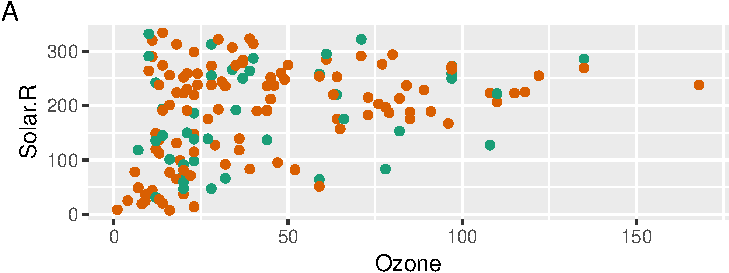
\includegraphics[width=1\linewidth]{tidy-missing-data-paper_files/figure-latex/track-impute-example-1} 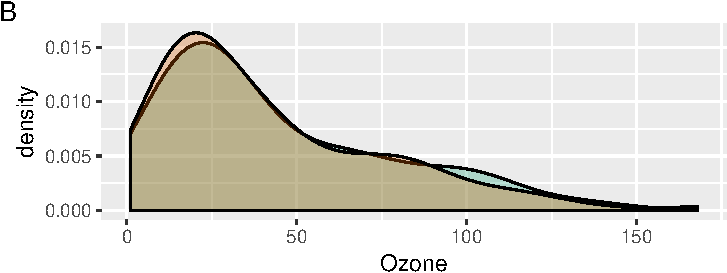
\includegraphics[width=1\linewidth]{tidy-missing-data-paper_files/figure-latex/track-impute-example-2} 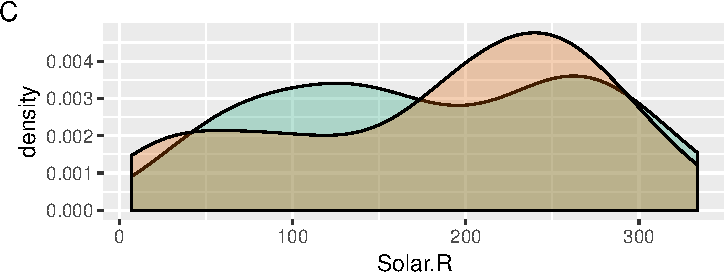
\includegraphics[width=1\linewidth]{tidy-missing-data-paper_files/figure-latex/track-impute-example-3} 

}

\caption{Scatterplot (A) and density plots (B and C) of ozone and solar radiation from the airquality dataset containing imputed values imputed using simputations `impute\_knn` function, with imputed values colored green and data values orange. Imputed values are similar, but slightly different to existing data.}\label{fig:track-impute-example}
\end{figure}

Imputed values can also be compared to complete case data by grouping by
\texttt{any\_missing}, and then summarizing (Table
\ref{tab:impute-summary}).

\begin{Shaded}
\begin{Highlighting}[]
\NormalTok{aq_imputed }\OperatorTok
\StringTok{  }\KeywordTok{group_by}\NormalTok{(any_missing) }\OperatorTok
\StringTok{  }\KeywordTok{summarise_at}\NormalTok{(}\DataTypeTok{.vars =} \KeywordTok{vars}\NormalTok{(Ozone),}
               \DataTypeTok{.funs =} \KeywordTok{funs}\NormalTok{(min, mean, median, max))}
\end{Highlighting}
\end{Shaded}

\begin{table}[!h]

\caption{\label{tab:impute-summary}Summary statistics of the previously imputed and complete cases. The mean and median values are similar, but the minimum and maximum values are different. The comparison of imputed values is similar to other dplyr summary workflows.}
\centering
\begin{tabular}[t]{lrrrr}
\toprule
any\_missing & min & mean & median & max\\
\midrule
Missing & 7 & 43.6 & 30 & 135\\
Not Missing & 1 & 42.1 & 31 & 168\\
\bottomrule
\end{tabular}
\end{table}

\hypertarget{case-study}{%
\section{Application}\label{case-study}}

To illustrate the methods, data on housing for the city of Melbourne
from January 28, 2016 to March 17, 2018 is used. The data was compiled
by scraping weekly property clearance data (Pino 2018). There are 27,247
properties, and 21 variables in the dataset. The variables include the
type of real estate (town house, unit, house), suburb, method of
selling, number of rooms, price, real estate agent, date of sale, and
the distance from the Central Business District (CBD).

The goal in analyzing this data is to accurately predict Melbourne
housing prices. The data contains many missing values. As a precursor to
building a predictive model, this analysis focusses on understanding the
patterns of missingness. This section shows how the methods from
previous sections are used together in a data analysis workflow.

\hypertarget{case-study-explore-pattern}{%
\subsection{Exploring patterns of
missingness}\label{case-study-explore-pattern}}

Figure \ref{fig:housing-miss-case-var}A shows 9 variables with missing
values. The most missings are in building area, followed by year built,
and land size, with similar amounts of missingness in Car, bathroom,
bedroom2, longitude, and latitude. Figure
\ref{fig:housing-miss-case-var}B reveals there are up to 50\% missing
values in cases, and that the majority of cases have more than 5\%
values missing. The variables building area and year built have more
than 50\% missing data, and so could perhaps be omitted from subsequent
analysis, as imputed values are likely to be spurious.

\begin{figure}

{\centering 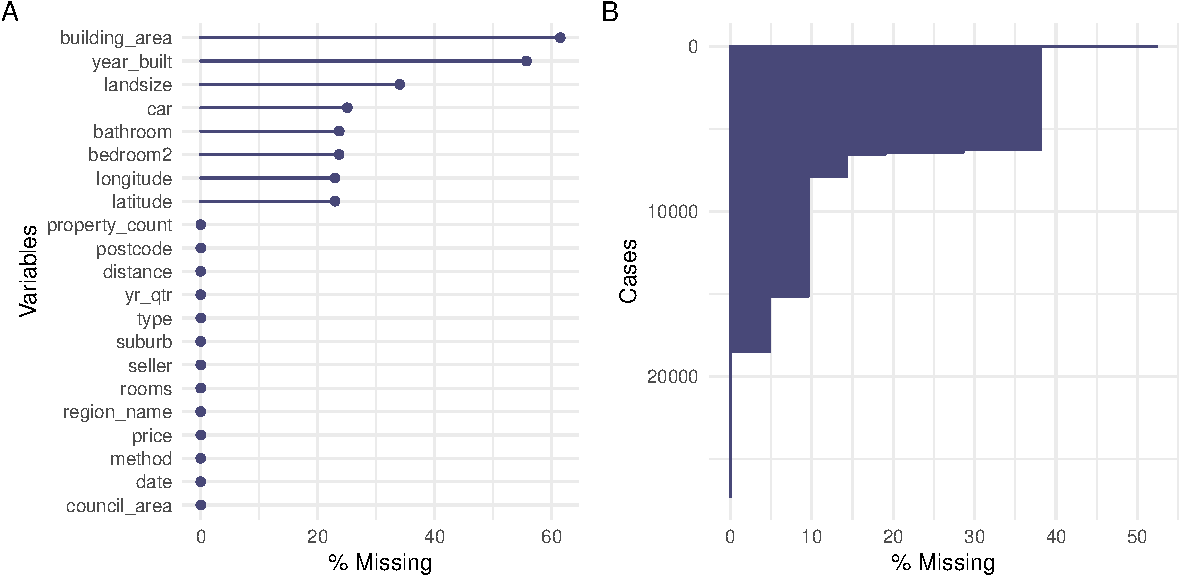
\includegraphics[width=1\linewidth]{tidy-missing-data-paper_files/figure-latex/housing-miss-case-var-1} 

}

\caption{The amount of missings in each variable (A) and in each case (B) for Melbourne housing data. (A) Build area and year built have more than 50\% missing values, and car, bathroom, bedroom2 and longitude and latitude have about 25\% missings. (B) There are between 5 and 50\% missing values in cases. There are many missing values in the data, with the majority of missingness being in selected cases and variables.}\label{fig:housing-miss-case-var}
\end{figure}

Possible missingness structures are revealed by visualizing missingness
in the whole dataset, clustering and arranging the rows and columns of
the data (Figure \ref{fig:applic-vis-miss}). There are three main
clusters of missing data: at the top there are many variables missing
together; in the middle, building price and year built missing together,
at the bottom, building area, year built, and land size are missing.

\begin{figure}

{\centering 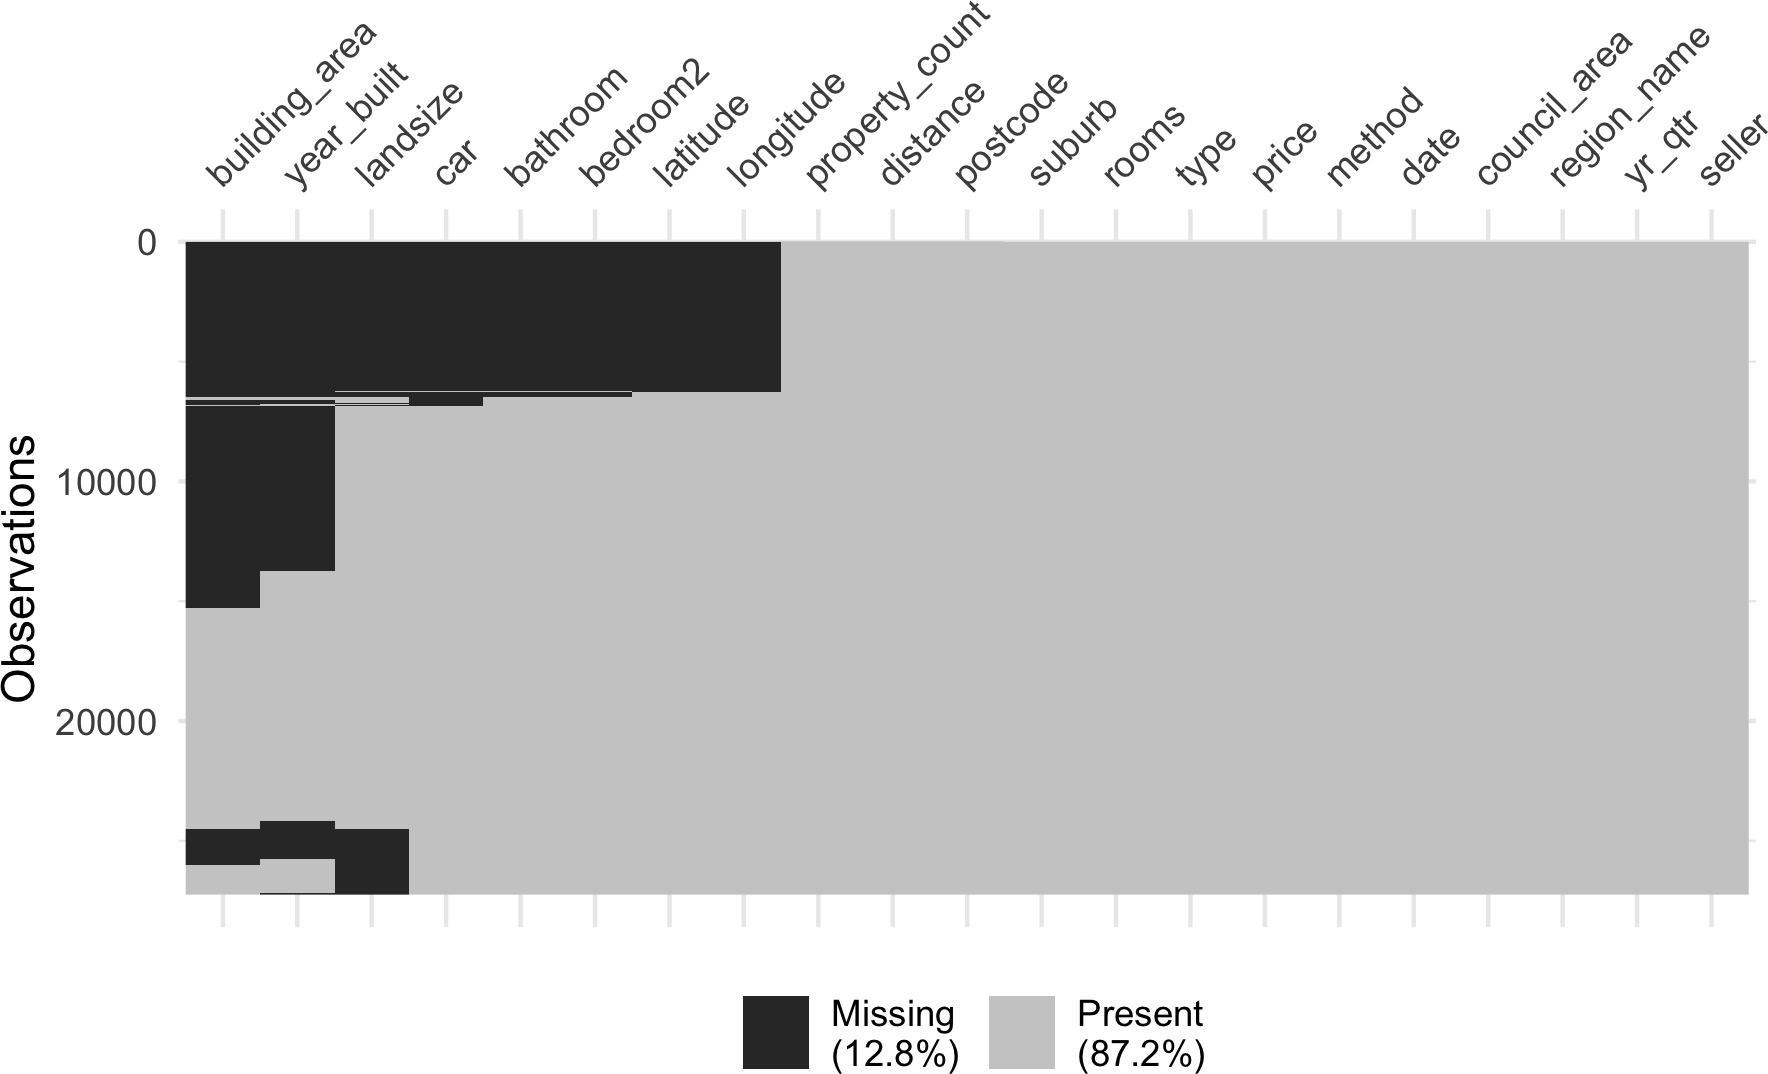
\includegraphics[width=0.85\linewidth]{tidy-missing-data-paper_files/figure-latex/applic-vis-miss-1} 

}

\caption{Heatmap of clustered missingness for the housing data. Three groups of missingness are apparent, at the top for building area to longitude, the middle for building area and year built, at the end for building area, year built, and landsize. There is some structure in the missings.}\label{fig:applic-vis-miss}
\end{figure}

Missingness patterns can also be shown with an \texttt{upset} plot
(Conway et al. 2017), to display the 8 of intersecting sets of missing
variables (see Figure \ref{fig:applic-vis-miss}. Two patterns stand out:
two, and five variables missing. This provides further evidence of the
patterns of missingness seen in Figures \ref{fig:housing-miss-case-var}
and \ref{fig:housing-upset}.

\begin{figure}

{\centering 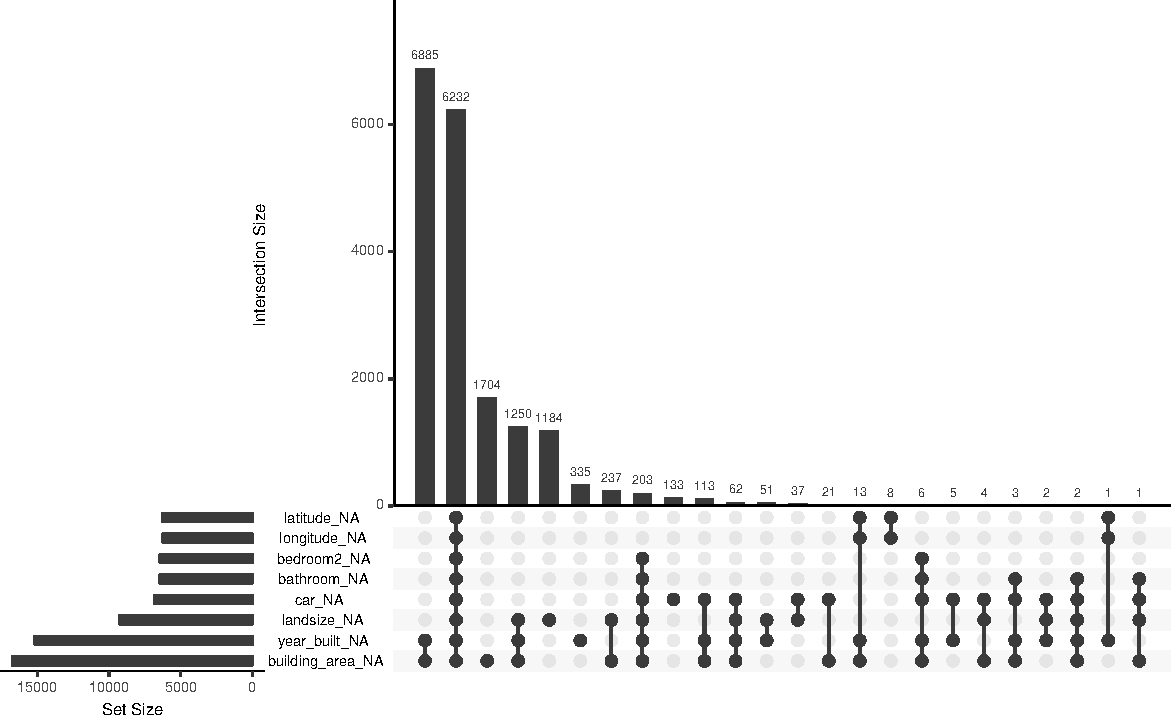
\includegraphics[width=1\linewidth]{tidy-missing-data-paper_files/figure-latex/housing-upset-1} 

}

\caption{An upset plot of eight sets of missingness in the housing data. Two missingness patterns are clear, year built and building area, and lattitude through to building area.}\label{fig:housing-upset}
\end{figure}

Tabulating the number of missings in variables (see Table
\ref{tab:housing-miss-var-case-table} (left)) shows three groupings:
6254 - 6824 missings cases in variables, 9265 in another variable, and
between 15163 and 16736 missing. Tabulating missings in cases (Table
\ref{tab:housing-miss-var-case-table} (right)) shows 32\% of cases have
complete data, 26\% have 2 missing, 22\% have 8 missing, 12\% have 1
missing, and 5\% have 3 missing, the remaining cases with missings are
less than 1\%. Two variables with more than 50\% missingness are omitted
from analysis: building area and year built.

\begin{table}[!h]
\caption{\label{tab:housing-miss-var-case-table}Tabulating missingness for variables (left) and cases (right) to understand missingness patterns. 14 variables have between 0 and 3 missings, then 6 variables have 6000 - 9000 missings, and 2 variables have 15 - 16,000 missing values. About 30\% of cases have no missing values, then 45\% of cases have between 1 and 6 missing values, and then about 23\% of cases have 8 or more missings. There are different patterns of missingness in variables and cases, but they can be broken down into smaller groups.}

\centering
\begin{tabular}[t]{rrr}
\toprule
n\_miss\_in\_var & n\_vars & pct\_vars\\
\midrule
0 & 10 & 47.6\\
1 & 2 & 9.5\\
3 & 1 & 4.8\\
6254 & 2 & 9.5\\
6441 & 1 & 4.8\\
\addlinespace
6447 & 1 & 4.8\\
6824 & 1 & 4.8\\
9265 & 1 & 4.8\\
15163 & 1 & 4.8\\
16736 & 1 & 4.8\\
\bottomrule
\end{tabular}
\centering
\begin{tabular}[t]{rrr}
\toprule
n\_miss\_in\_case & n\_cases & pct\_cases\\
\midrule
0 & 8755 & 32.1\\
1 & 3356 & 12.3\\
2 & 7244 & 26.6\\
3 & 1370 & 5.0\\
4 & 79 & 0.3\\
\addlinespace
5 & 8 & 0.0\\
6 & 203 & 0.7\\
8 & 6229 & 22.9\\
9 & 2 & 0.0\\
11 & 1 & 0.0\\
\bottomrule
\end{tabular}
\end{table}

\hypertarget{case-study-explore-for-imp}{%
\subsection{Exploring missingness patterns for
imputation}\label{case-study-explore-for-imp}}

Using the information from the overview visualizations and tables, the
following variables are explored for features predicting missingness:
Land size, latitude, longitude, bedroom2, bathroom, car, and land size.

Missingness structure can be better understood and evaluated by using
the data to predict where the data goes missing. This can be achieved by
clustering the missing values into groups, and then applying
classification and regression trees (CART) to find those variables and
values that predict missingness clusters (Barnett et al. 2017; Tierney
et al. 2015). Two clusters are identified, one for each missingness
cluster. The missingness clusters are predicted using all variables in
the dataset with the CART package \texttt{rpart} (Therneau and Atkinson
2018), and plotted using the \texttt{rpart.plot} package (Milborrow
2018). Importance scores from the CART model describe those variables
important for predicting missingness: rooms, price, suburb, council
area, distance, and region name. These variables are important for
predicting missingness, so are important to include in the imputation
model.

\begin{figure}

{\centering 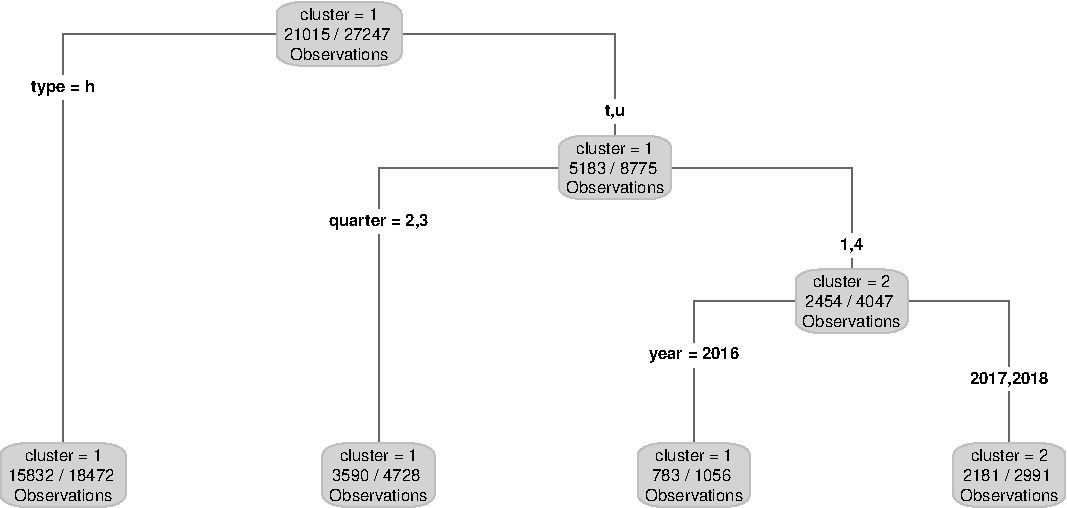
\includegraphics[width=1\linewidth]{tidy-missing-data-paper_files/figure-latex/rpart-plot-1} 

}

\caption{Decision tree output predicting the clusters of missingness. Type of house, the year quarter, and year were important for predicting missingness cluster. The cluster with the most missingness was for quarters 1 and 4, for 2017 and 2018. Type of house, year, and year quarter are important features related to the missingness structure.}\label{fig:rpart-plot}
\end{figure}

\hypertarget{case-study-imp-diagnosis}{%
\subsection{Imputation and diagnostics}\label{case-study-imp-diagnosis}}

Two different imputation techniques are used: simple linear regression
and K nearest neighbors. Values are imputed stepwise in ascending order
of missingness. The \texttt{simputation} R package (van der Loo 2017) is
used to impute the values, applying the track missings pattern described
in Section \ref{verbs-track}, to assess imputed values.

Imputed data are combined by row binding imputation models. The data are
reshaped into long format to compare imputed values for each model for 4
variables (Figure \ref{fig:imputed-by-model}). Compared to KNN imputed
values, the linear model imputed values closer to the mean value.

\begin{figure}

{\centering 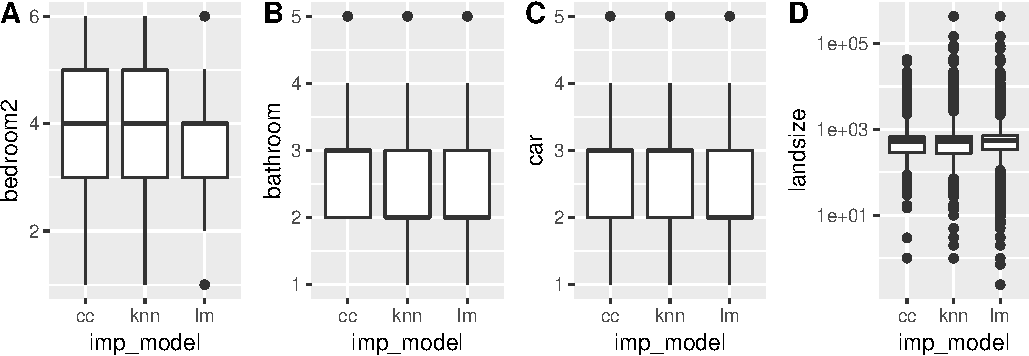
\includegraphics[width=0.95\linewidth]{tidy-missing-data-paper_files/figure-latex/imputed-by-model-1} 

}

\caption{Boxplots of complete case data, and data imputed with KNN or linear model for different variables. (A) number of bedrooms, (B) number of bathrooms, (C) number of carspots, and (D) landsize (on a log10 scale). KNN had similar results to complete case, and linear model had a lower median for cars and fewer extreme values for bedrooms.}\label{fig:imputed-by-model}
\end{figure}

\hypertarget{case-study-assess-model}{%
\subsection{Assess model predictions}\label{case-study-assess-model}}

The coefficients of the linear model of log price vary for room (Figure
\ref{fig:tidy-coefs}), for different imputed datasets. Notably, complete
cases resulted in underestimating the impact of room on log price. A
partial residual plot (Figure \ref{fig:partial-resid}) shows there is
not much variation amongst the models from the different datasets.

\begin{figure}

{\centering 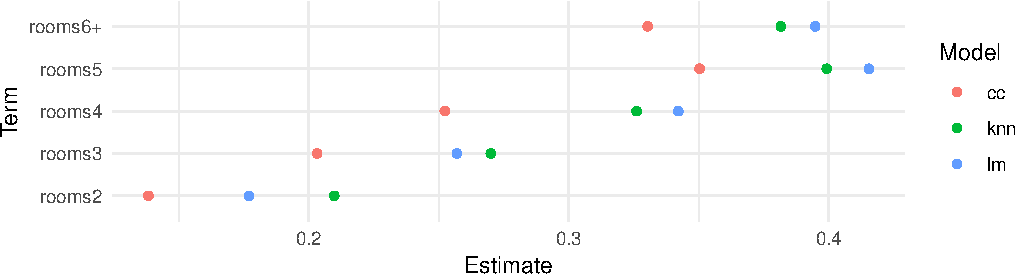
\includegraphics[width=1\linewidth]{tidy-missing-data-paper_files/figure-latex/tidy-coefs-1} 

}

\caption{Visualization of the variation in coefficients for linear model of log price for each of the different datasets for the number of rooms. In red is complete case (cc), in green is the knn imputed dataset, and in blue the imputed by linear model. Using the complete case dataset produced smaller coefficients compared to the imputed models.}\label{fig:tidy-coefs}
\end{figure}

\begin{figure}

{\centering 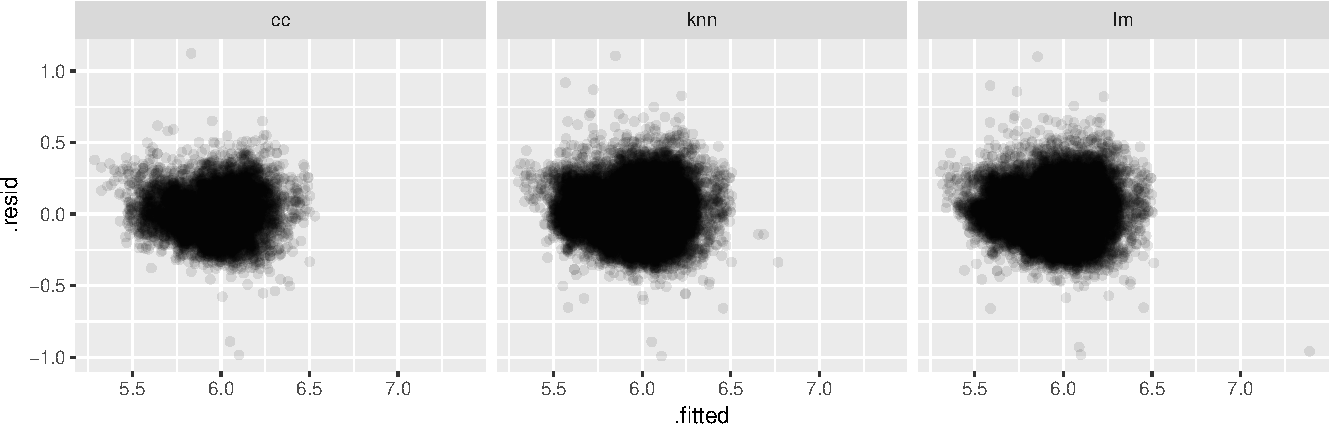
\includegraphics[width=1\linewidth]{tidy-missing-data-paper_files/figure-latex/partial-resid-1} 

}

\caption{Partial residual plot for each data set, complete cases (cc), imputed with KNN (knn), and imputed with a linear model (lm). There is not much variation amongst the different datasets from the different imputation methods.}\label{fig:partial-resid}
\end{figure}

\hypertarget{case-study-summary}{%
\subsection{Summary}\label{case-study-summary}}

The \texttt{naniar} and \texttt{visdat} packages build on existing tidy
tools and strike a compromise between automation and control that makes
analysis efficient, readable, but not overly complex. Each tool has
clear intent and effects - plotting or generating data or augmenting
data in some way. This reduces repetition and typing for the user,
making exploration of missing values easier as they follow consistent
rules with a declarative interface.

\hypertarget{discussion}{%
\section{Discussion}\label{discussion}}

This paper has described new methods for exploring, visualizing, and
imputing missing data. The work was motivated by recent developments of
tidy data, and extends them for better missing value handling. The
methods have standard outputs, function arguments, and behavior. This
provides consistent workflows centered around data analysis that
integrate well with existing imputation methodology, visualization, and
modelling.

The new data structures discussed in the paper could be used to create
different visualizations than were shown in the paper. The analyst can
use the data structures to decide on appropriate visualization for their
problem. The data structures could also be used to support interactive
graphics, in the manner of MANET and ggobi. Linking the plots (linked
brushing) to explore missingness or animating between different sets of
imputed values. New packages like \texttt{plotly} (Sievert 2018)
facilitate interactive graphics, and packages like \texttt{gganimate}
facilitate animations (Pedersen and Robinson 2017).

Other data structures such as spatial data, time series, networks, and
longitudinal data would be supported by the inherently tabular,
\emph{nabular} data, if they are first structured as wide tidy format.
Large data may need special handling, and additional features like
efficient storage of purely imputed values and lazy evaluation. Special
missing value codes could be improved by creating special classes, or
expanding low level representation of \texttt{NA} at the source code
level.

The methodology described in this paper can be used in conjunction with
other approaches to understand multivariate missingness dependencies
(e.g.~decision trees (Tierney et al. 2015), latent group analysis
(Barnett et al. 2017), and PCA (Lê et al. 2008)) . Evaluating imputed
values using a testing framework like Buuren (2012) is also supported.

The approach meshes with the dynamic nature of data analysis, allowing
the analyst to go from raw data to model data in a fluid workflow.

\newpage

\hypertarget{acknowledgements}{%
\section{Acknowledgements}\label{acknowledgements}}

The authors would like to thank Miles McBain, for his key contributions
and discussions on the \texttt{naniar} package, in particular for
helping implement \texttt{geom\_miss\_point}, and for his feedback on
ideas, implementations, and names. We also thank Colin Fay for his
contributions to the \texttt{naniar} package, in particular for his
assistance with the \texttt{replace\_with\_na} functions. We also thank
Earo Wang and Mitchell O'Hara-Wild for the many useful discussions on
missing data and package development, and for their assistance with
creating elegant approaches that take advantage of the tidy syntax. We
would also like to thank those who contributed pull requests and
discussions on the \texttt{naniar} package, in particular Jim Hester and
Romain François for improving the speed of key functions, Ross Gayler
for discussion on special missing values, and Luke Smith for helping
\texttt{naniar} be more compliant with \texttt{ggplot2}.

\hypertarget{references}{%
\section*{References}\label{references}}
\addcontentsline{toc}{section}{References}

\hypertarget{refs}{}
\leavevmode\hypertarget{ref-Barnett2017}{}%
Barnett, A. G., McElwee, P., Nathan, A., Burton, N. W., and Turrell, G.
(2017), ``Identifying patterns of item missing survey data using latent
groups: An observational study,'' \emph{BMJ open}, bmjopen.bmj.com, 7,
e017284.

\leavevmode\hypertarget{ref-Broman2017}{}%
Broman, K. W., and Woo, K. H. (2017), \emph{Data organization in
spreadsheets}, PeerJ Preprints; PeerJ Inc.

\leavevmode\hypertarget{ref-VanBuuren2012}{}%
Buuren, S. van (2012), \emph{Flexible imputation of missing data}, CRC
Press.

\leavevmode\hypertarget{ref-Cheng2015}{}%
Cheng, X., Cook, D., and Hofmann, H. (2015), ``Visually exploring
missing values in multivariable data using a graphical user interface,''
\emph{Journal of statistical software}, 68, 1--23.

\leavevmode\hypertarget{ref-Conway2017}{}%
Conway, J. R., Lex, A., and Gehlenborg, N. (2017), ``UpSetR: An R
package for the visualization of intersecting sets and their
properties,'' \emph{Bioinformatics}, 33, 2938--2940.

\leavevmode\hypertarget{ref-Cook2007}{}%
Cook, D., and Swayne, D. F. (2007), \emph{Interactive and dynamic
graphics for data analysis with R and GGobi}, Springer Publishing
Company, Incorporated.

\leavevmode\hypertarget{ref-Dempster1977}{}%
Dempster, A. P., Laird, N. M., and Rubin, D. B. (1977), ``Maximum
likelihood from incomplete data via the EM algorithm,'' \emph{Journal of
the Royal Statistical Society. Series B, Statistical methodology},
{[}Royal Statistical Society, Wiley{]}, 39, 1--38.

\leavevmode\hypertarget{ref-Donoho2017}{}%
Donoho, D. (2017), ``50 years of data science,'' \emph{Journal of
computational and graphical statistics: a joint publication of American
Statistical Association, Institute of Mathematical Statistics, Interface
Foundation of North America}, Taylor \& Francis, 26, 745--766.

\leavevmode\hypertarget{ref-Durre2008-ghcn}{}%
Durre, I., Menne, M. J., and Vose, R. S. (2008), ``Strategies for
evaluating quality assurance procedures,'' \emph{Journal of Applied
Meteorology and Climatology}, American Meteorological Society, 47,
1785--1791.

\leavevmode\hypertarget{ref-Ellis2017}{}%
Ellis, S. E., and Leek, J. T. (2017), \emph{How to share data for
collaboration}, PeerJ Preprints; PeerJ Inc.

\leavevmode\hypertarget{ref-mi}{}%
Gelman, A., and Hill, J. (2011), ``Opening windows to the black box,''
\emph{Journal of Statistical Software}, 40.

\leavevmode\hypertarget{ref-lubridate}{}%
Grolemund, G., and Wickham, H. (2011), ``Dates and times made easy with
lubridate,'' \emph{Journal of Statistical Software}, 40, 1--25.

\leavevmode\hypertarget{ref-Hmisc}{}%
Harrell Jr, F. E., Charles Dupont, and others. (2018), \emph{Hmisc:
Harrell miscellaneous}.

\leavevmode\hypertarget{ref-purrr}{}%
Henry, L., and Wickham, H. (2017), \emph{Purrr: Functional programming
tools}.

\leavevmode\hypertarget{ref-Honaker2010}{}%
Honaker, J., and King, G. (2010), ``What to do about missing values in
Time-Series Cross-Section data,'' \emph{American journal of political
science}, 54, 561--581.

\leavevmode\hypertarget{ref-amelia}{}%
Honaker, J., King, G., and Blackwell, M. (2011), ``Amelia II: A program
for missing data,'' \emph{Journal of Statistical Software}, 45, 1--47.

\leavevmode\hypertarget{ref-missMDA}{}%
Josse, J., and Husson, F. (2016), ``MissMDA: A package for handling
missing values in multivariate data analysis,'' \emph{Journal of
Statistical Software, Articles}, 70, 1--31.
\url{https://doi.org/10.18637/jss.v070.i01}.

\leavevmode\hypertarget{ref-Keeling2005-scripps}{}%
Keeling, C. D., Piper, S. C., Bacastow, R. B., Wahlen, M., Whorf, T. P.,
Heimann, M., and Meijer, H. A. (2005), ``Atmospheric CO2 and 13CO2
exchange with the terrestrial biosphere and oceans from 1978 to 2000:
Observations and carbon cycle implications,'' in \emph{A history of
atmospheric CO2 and its effects on plants, animals, and ecosystems},
eds. I. T. Baldwin, M. M. Caldwell, G. Heldmaier, R. B. Jackson, O. L.
Lange, H. A. Mooney, E.-D. Schulze, U. Sommer, J. R. Ehleringer, M.
Denise Dearing, and T. E. Cerling, New York, NY: Springer New York, pp.
83--113.

\leavevmode\hypertarget{ref-VIM}{}%
Kowarik, A., and Templ, M. (2016), ``Imputation with the R package
VIM,'' \emph{Journal of Statistical Software}, 74, 1--16.
\url{https://doi.org/10.18637/jss.v074.i07}.

\leavevmode\hypertarget{ref-recipes}{}%
Kuhn, M., and Wickham, H. (2018), \emph{Recipes: Preprocessing tools to
create design matrices}.

\leavevmode\hypertarget{ref-FactoMineR}{}%
Lê, S., Josse, J., and Husson, F. (2008), ``FactoMineR: A package for
multivariate analysis,'' \emph{Journal of Statistical Software}, 25,
1--18. \url{https://doi.org/10.18637/jss.v025.i01}.

\leavevmode\hypertarget{ref-Little1988}{}%
Little, R. J. A. (1988), ``A test of missing completely at random for
multivariate data with missing values,'' \emph{Journal of the American
Statistical Association}, Taylor \& Francis, 83, 1198--1202.

\leavevmode\hypertarget{ref-rpart-plot}{}%
Milborrow, S. (2018), \emph{Rpart.plot: Plot 'rpart' models: An enhanced
version of 'plot.rpart'}.

\leavevmode\hypertarget{ref-imputeTS}{}%
Moritz, S., and Bartz-Beielstein, T. (2017), ``imputeTS: Time Series
Missing Value Imputation in R,'' \emph{The R Journal}, 9, 207--218.

\leavevmode\hypertarget{ref-gganimate}{}%
Pedersen, T. L., and Robinson, D. (2017), \emph{Gganimate: A grammar of
animated graphics}.

\leavevmode\hypertarget{ref-kaggle2018}{}%
Pino, T. (2018), ``Melbourne housing market,''
\url{https://www.kaggle.com/anthonypino/melbourne-housing-market/version/21}.

\leavevmode\hypertarget{ref-norm}{}%
R by Alvaro A. Novo. Original by Joseph L. Schafer
\textless{}jls@stat.psu.edu\textgreater{}., P. to (2013), \emph{Norm:
Analysis of multivariate normal datasets with missing values}.

\leavevmode\hypertarget{ref-Ross2017}{}%
Ross, Z., Wickham, H., and Robinson, D. (2017), \emph{Declutter your R
workflow with tidy tools}, PeerJ Preprints; PeerJ Inc.

\leavevmode\hypertarget{ref-Rubin1976}{}%
Rubin, D. B. (1976), ``Inference and missing data,'' \emph{Biometrika},
Oxford University Press, 63, 581--592.

\leavevmode\hypertarget{ref-schafer-norm}{}%
Schafer, J. (1999), \emph{NORM: Multiple imputation of incomplete
multivariate data under a normal model}, University Park: Pennsylvania
State University, Department of Statistics.

\leavevmode\hypertarget{ref-Schafer2002}{}%
Schafer, J. L., and Graham, J. W. (2002), ``Missing data: Our view of
the state of the art,'' \emph{Psychological methods}, 7, 147--177.

\leavevmode\hypertarget{ref-plotly}{}%
Sievert, C. (2018), \emph{Plotly for r}.

\leavevmode\hypertarget{ref-tidytext}{}%
Silge, J., and Robinson, D. (2016), ``Tidytext: Text mining and analysis
using tidy data principles in r,'' \emph{JOSS}, The Open Journal, 1.
\url{https://doi.org/10.21105/joss.00037}.

\leavevmode\hypertarget{ref-Simon1986}{}%
Simon, G. A., and Simonoff, J. S. (1986), ``Diagnostic plots for missing
data in least squares regression,'' \emph{Journal of the American
Statistical Association}, Taylor \& Francis, 81, 501--509.

\leavevmode\hypertarget{ref-Sterne2009}{}%
Sterne, J. a C., White, I. R., Carlin, J. B., Spratt, M., Royston, P.,
Kenward, M. G., Wood, A. M., and Carpenter, J. R. (2009), ``Multiple
imputation for missing data in epidemiological and clinical research:
Potential and pitfalls,'' \emph{BMJ}, 338, b2393.

\leavevmode\hypertarget{ref-Swayne1998}{}%
Swayne, D. F., and Buja, A. (1998), ``Missing data in interactive
high-dimensional data visualization,'' \emph{Computational statistics},
researchgate.net, 1--8.

\leavevmode\hypertarget{ref-rpart}{}%
Therneau, T., and Atkinson, B. (2018), \emph{Rpart: Recursive
partitioning and regression trees}.

\leavevmode\hypertarget{ref-visdat}{}%
Tierney, N. (2017), ``Visdat: Visualising whole data frames,''
\emph{JOSS}, Journal of Open Source Software, 2, 355.
\url{https://doi.org/10.21105/joss.00355}.

\leavevmode\hypertarget{ref-Tierney2015}{}%
Tierney, N. J., Harden, F. A., Harden, M. J., and Mengersen, K. L.
(2015), ``Using decision trees to understand structure in missing
data,'' \emph{BMJ open}, bmjopen.bmj.com, 5, e007450.

\leavevmode\hypertarget{ref-treisman1985}{}%
Treisman, A. (1985), ``Preattentive processing in vision,''
\emph{Computer vision, graphics, and image processing}, 31, 156--177.

\leavevmode\hypertarget{ref-Unwin1996}{}%
Unwin, A., Hawkins, G., Hofmann, H., and Siegl, B. (1996), ``Interactive
graphics for data sets with missing values: MANET,'' \emph{Journal of
computational and graphical statistics: a joint publication of American
Statistical Association, Institute of Mathematical Statistics, Interface
Foundation of North America}, {[}American Statistical Association,
Taylor \& Francis, Ltd., Institute of Mathematical Statistics, Interface
Foundation of America{]}, 5, 113--122.

\leavevmode\hypertarget{ref-mice}{}%
van Buuren, S., and Groothuis-Oudshoorn, K. (2011), ``mice: Multivariate
imputation by chained equations in r,'' \emph{Journal of Statistical
Software}, 45, 1--67.

\leavevmode\hypertarget{ref-simputation}{}%
van der Loo, M. (2017), \emph{Simputation: Simple imputation}.

\leavevmode\hypertarget{ref-tidycensus}{}%
Walker, K. (2018), \emph{Tidycensus: Load us census boundary and
attribute data as 'tidyverse' and 'sf'-ready data frames}.

\leavevmode\hypertarget{ref-tsibble}{}%
Wang, E., Cook, D., and Hyndman, R. (2018), \emph{Tsibble: Tidy temporal
data frames and tools}.

\leavevmode\hypertarget{ref-ggplot2}{}%
Wickham, H. (2009), \emph{Ggplot2: Elegant graphics for data analysis},
Springer-Verlag New York.

\leavevmode\hypertarget{ref-Wickham2014}{}%
Wickham, H. (2014), ``Tidy data,'' \emph{Journal of statistical
software}, 59, 1--23.

\leavevmode\hypertarget{ref-Tidyverse-Manifesto}{}%
Wickham, H. (2017), ``The tidy tools manifesto,''
\url{https://cran.r-project.org/web/packages/tidyverse/vignettes/manifesto.html}.

\leavevmode\hypertarget{ref-stringr}{}%
Wickham, H. (2018), \emph{Stringr: Simple, consistent wrappers for
common string operations}.

\leavevmode\hypertarget{ref-readxl}{}%
Wickham, H., and Bryan, J. (2017), \emph{Readxl: Read excel files}.

\leavevmode\hypertarget{ref-dplyr}{}%
Wickham, H., Francois, R., Henry, L., and Müller, K. (2017a),
\emph{Dplyr: A grammar of data manipulation}.

\leavevmode\hypertarget{ref-r4ds}{}%
Wickham, H., and Grolemund, G. (2016), \emph{R for data science: Import,
tidy, transform, visualize, and model data}, ``O'Reilly Media, Inc.''.

\leavevmode\hypertarget{ref-tidyr}{}%
Wickham, H., and Henry, L. (2018), \emph{Tidyr: Easily tidy data with
'spread()' and 'gather()' functions}.

\leavevmode\hypertarget{ref-readr}{}%
Wickham, H., Hester, J., and Francois, R. (2017b), \emph{Readr: Read
rectangular text data}.

\leavevmode\hypertarget{ref-haven}{}%
Wickham, H., and Miller, E. (2018), \emph{Haven: Import and export
'spss', 'stata' and 'sas' files}.


\end{document}
